
\documentclass[a4paper,12pt]{article}
\usepackage{graphicx}
\usepackage[table,xcdraw]{xcolor}
\usepackage{geometry}
\usepackage{float}
\usepackage[colorlinks=false, hidelinks]{hyperref}
\usepackage{fancyhdr}% For page numbering
\geometry{top=1in,bottom=1in,left=1in,right=1in}
\usepackage{listings}
\usepackage{xcolor}
\usepackage{hyperref}
\pagestyle{empty}


\begin{document}

\begin{center}
    \vspace{0.2cm}
    \textbf{\large{Course Title: Software Engineering \& ISD Lab}}\\
    \vspace{0.2cm}
    \textbf{Course Code: CSE-404}\\
    \vspace{0.2cm}
    \textbf{4\textsuperscript{th}Year 1\textsuperscript{st}Semester Examination 2023}\\
    \vspace{0.5cm}
    \textbf{Date of Submission: \today}\\

    \vspace{1.5cm}
    
\includegraphics[width=0.35\textwidth]{images/logo.png}\\ % Replace 'logo.png' with the correct path if you have the university logo image
    \vspace{1cm}

    \textbf{Submitted to}\\
    \vspace{0.2cm}
    \textbf{\href{https://juniv.edu/teachers/musfique.anwar}{Dr. Md Musfique Anwar}}\\
    {Professor}\\
    \vspace{0.2cm}
    \textbf{\href{https://juniv.edu/teachers/hkabir}{Dr. Md. Humayun Kabir}}\\
    {Professor}\\


    \vspace{1cm}

    \begin{table}[h!]
        \centering
        \arrayrulecolor{black}
        \begin{tabular}{|c|c|c|c|}
            \hline
            \rowcolor[HTML]{2F4F4F} % Changed header background color to dark slate gray
            {\color[HTML]{FFFFFF}\textbf{Sl}}& {\color[HTML]{FFFFFF}\textbf{Class Roll}}& {\color[HTML]{FFFFFF}\textbf{Exam Roll}}& {\color[HTML]{FFFFFF}\textbf{Name}}\\ \hline
            \rowcolor[HTML]{B0E0E6}
            \textbf{1}& \textbf{408} & \textbf{202220} & \textbf{Sudipta Singha} \\ \hline
       
        \end{tabular}
    \end{table}

    \vspace{1cm}

    Department of Computer Science and Engineering\\
    Jahangirnagar University\\
    Savar, Dhaka, Bangladesh\\
\end{center}

\newpage

\tableofcontents

\newpage
\pagestyle{fancy}
\fancyhf{}
\fancyfoot[C]{\thepage} % Page number in the center of the footer
\section{Introduction}
The Jahangirnagar University Medical Center Management System project was designed
to streamline and digitalize the management of the university’s medical center. This sys-
tem aimed to provide essential features such as user registration, appointment scheduling,
inventory tracking for the medical store, and the publication of informational vlogs on
seasonal diseases. The project’s primary objective was to enhance efficiency, improve
accessibility for users, and ensure better management of medical resources. During my
involvement, the project achieved several milestones, including a functional user authen-
tication system, a dynamic dashboard for doctors, lab technician, storekeeper users, and
the successful integration of ambulance driver details for emergency services. The project
utilized Django as the backend framework, ensuring a robust and scalable system. .
Github link for the project is provided here
\begin{figure}[H]
    \centering
    
\includegraphics[width=0.5\textwidth]{images/simple_prcode.png}
    \caption{QR code for the project link}
    \label{fig:qrcode}
\end{figure}
\textbf{Features}
\begin{itemize}
    \item Sign Up
    \item Log In
    \item See the information of waiting patients
    \item Prescribe medicines and test for a patient
    \item Dispense medicines to patients
    \item Update stock information
    \item Certify patients for fund collection
    \item Publish information and preventative measures for seasonal diseases
    \item Schedule appointment for doctors and lab tests
    \item Collect test reports and Prescriptions
    \item Reschedule test appointments
    \item Submit test reports
    \item Visit the seasonal diseases portal
\end{itemize}
\section{Sprint Overview}
In Sprint 2, we aimed to utilize the feedback and lessons learned from Sprint 1 to improve both the product
and our agile scrum processes. This included updating our product backlog, planning a new sprint backlog, and
incorporating Test-Driven Development (TDD) and continuous integration testing into our workflow. These
improvements were intended to enhance the quality of our deliverables and streamline our development
practices.
\section{Practice Improvement}
From Sprint-1 we identified potential improvement, which we will incorporate in our sprint 2. Those are
\begin{itemize}
    \item Better time tracking using toggl
    \item Using a proper gitignore for minimizing conflicts 
    \item Test Driven Development implementation and dashboard refinement are prioritized.
    \item Adjusted time estimates for complex tasks based on sprint 1 experience
\end{itemize}

\section{Meeting}
\subsection{Sprint 2 Planning Meeting}
To start the actual development phase of sprint
a team meeting was held.The main goal of the meeting is to establish the foundational elements of the Sprint. During the meeting, the following outcomes were achieved:
\begin{itemize}
    \item \textbf{Roles Assigned:}
        \begin{itemize}
            \item Product Owner: Hasan Al Mamun
            \item Scrum Master: \textbf{Sudipta Singha}
            \item Scrum Members:
                \begin{itemize}
                    \item Subarna Saha
                    \item Fatima Binte Aziz
                    \item Shabrina Akter Shahana
                    \item Saud Al Nahian

                \end{itemize}
        \end{itemize}

    \item \textbf{TDD:}\\We will follow Test Driven Development Approach in this sprint. That means test cases
        are written and implemented first. After test cases are generated actual feature implementation will
        start.
    \item \textbf{Sprint Backlog Agreement:}\\Tasks were selected and prioritized for Sprint 2 in consultation
        with the project owner.The tasks are also assigned to members. The Sprint 1 backlog which are decided are.
        \begin{enumerate}
            \item Prescribe Patients(Subarna Saha)
            \item Update Stock Information(Sudipta Singha)
            \item Collect test reports and Prescription(Fatima Binte Aziz)
            \item Certify for fundrise(Hasan Al Mamun)
            \item Submit test report(Shabrina Akter Shahana)
            \item Visit the seasonal disease porta(Saud Al Nahian)
        \end{enumerate}
        \item \textbf{Git Branch Name Convention: }\\Everyone will start working on the project in a branch named
        \textbf{branch-feature-member\_name\_initials} (e.g., branch-log-in-ss).
    \item \textbf{Git Commit Message Convention: }\\The format of the git commit messages was decided.
    \item \textbf{Discord Integration: } \\The decision to create a discord channel in our projects discord server to
        facilitate seamless communication during sprint 1 was taken.
    \item \textbf{Sprint Goals Defined: }The team agreed on the primary objectives and deliverables for Sprint
        2.
\end{itemize}
\newpage
\begin{figure}[H]
    \centering
    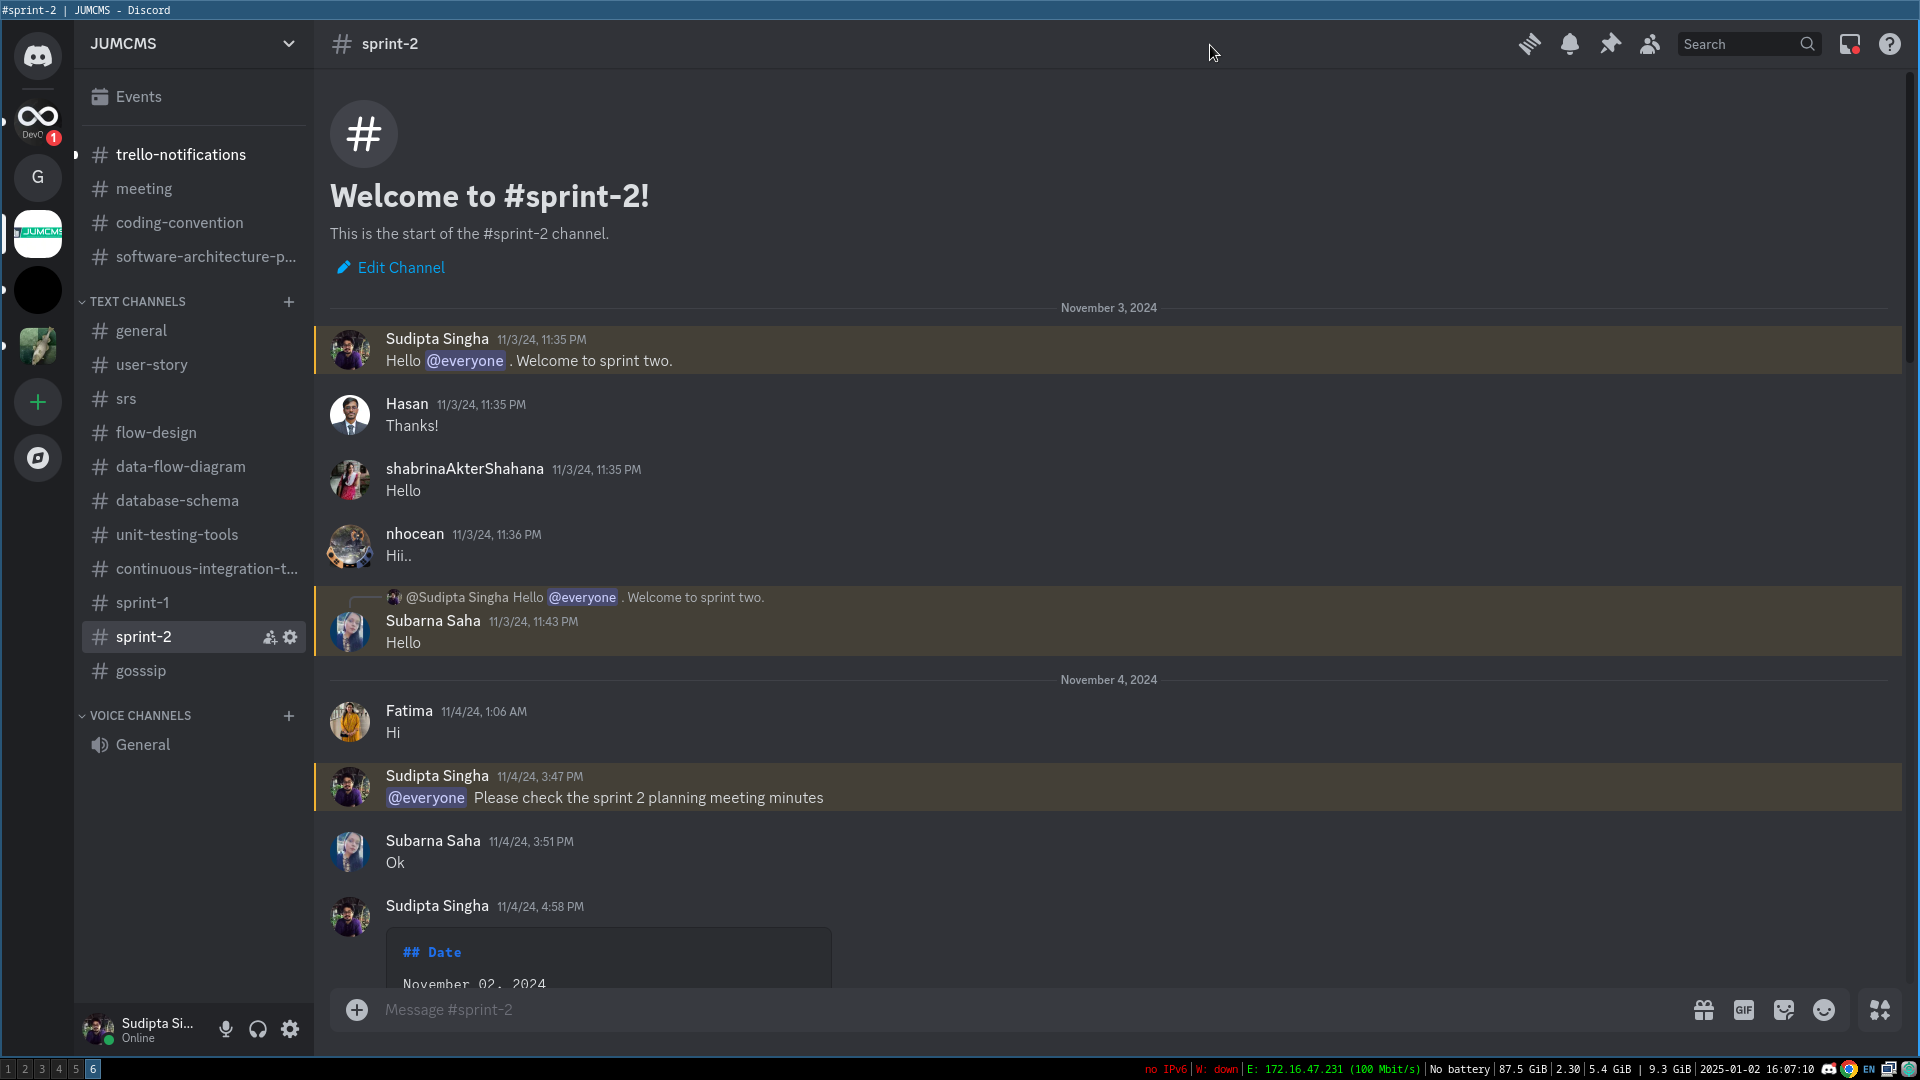
\includegraphics[width=1\textwidth]{images/spr2plan1.png}   
    \caption{Discord Server Creation}
    \label{fig:spr2plan1}
\end{figure}
\begin{figure}[H]
    \centering
    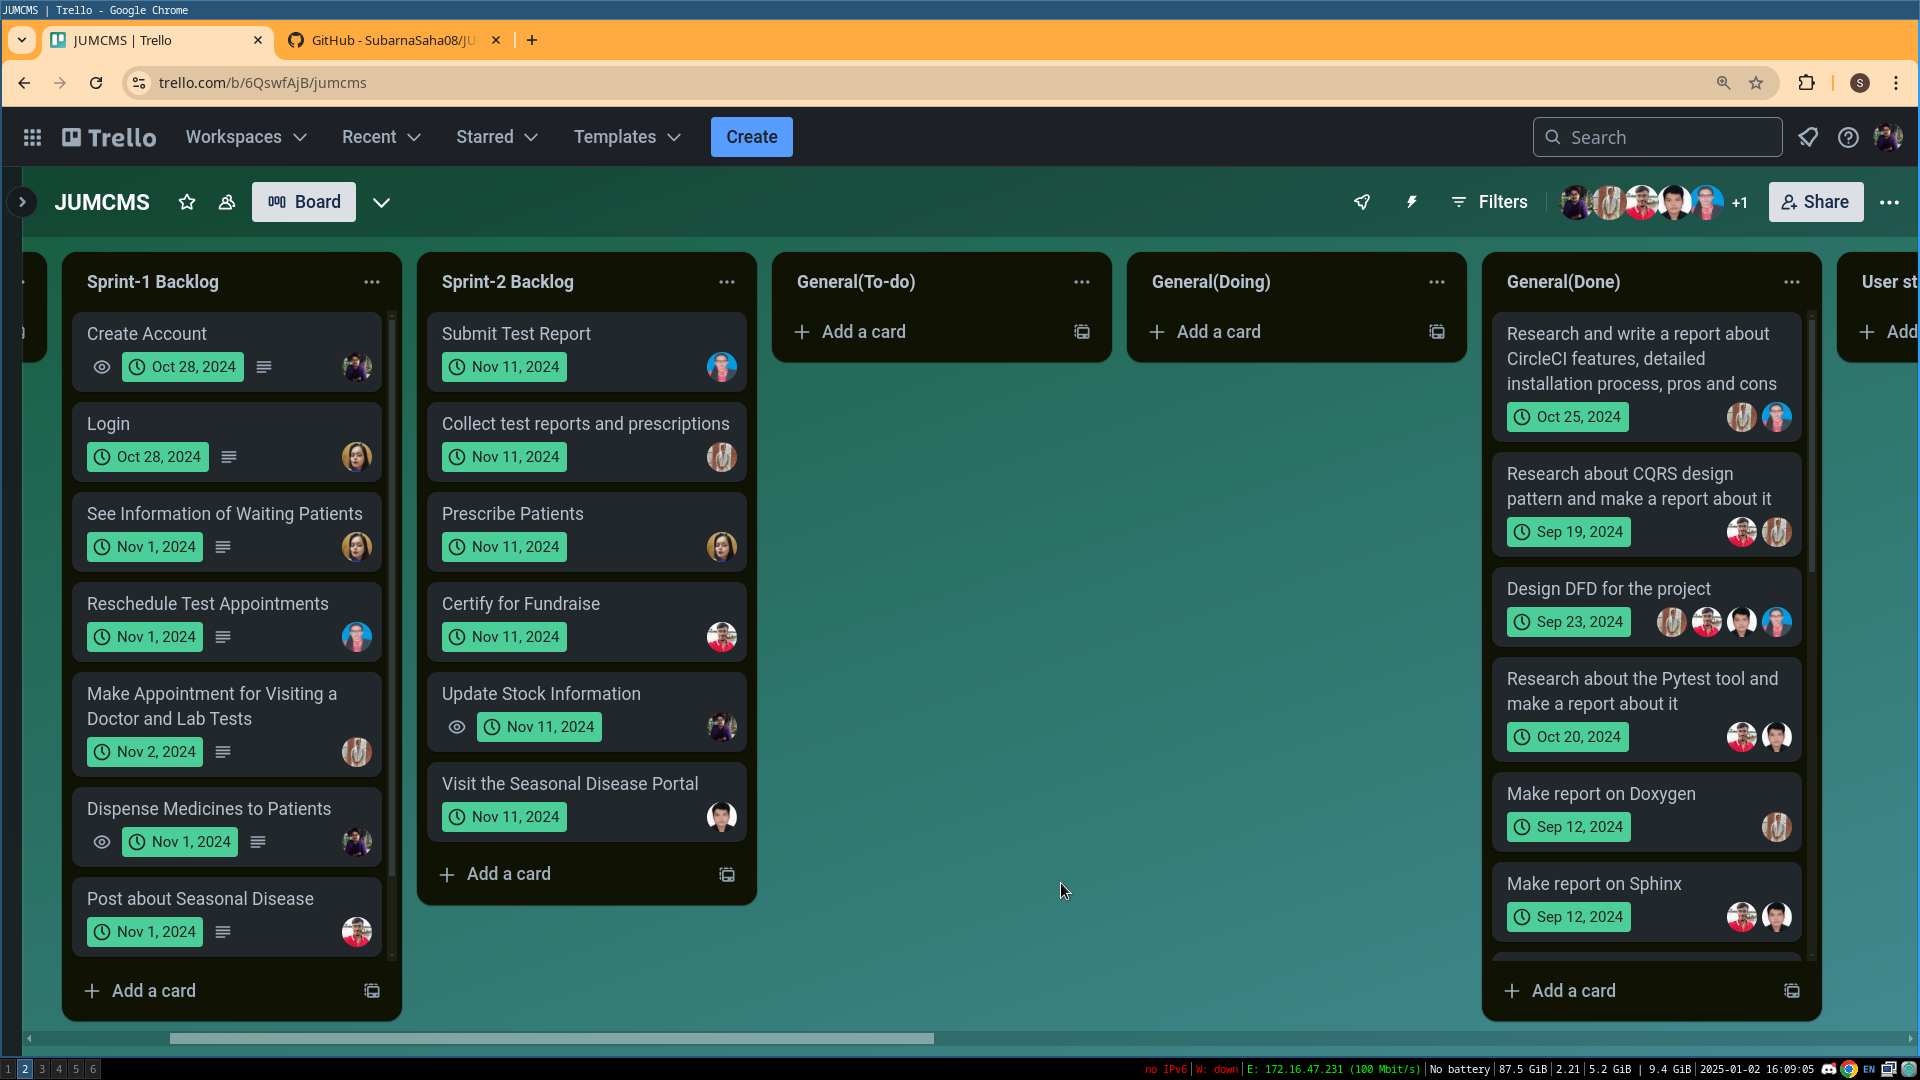
\includegraphics[width=1\textwidth]{images/spr2plan2.png}   
    \caption{Trello board for sprint 2}
    \label{fig:spr2plan2}
\end{figure}
\begin{figure}[H]
    \centering
    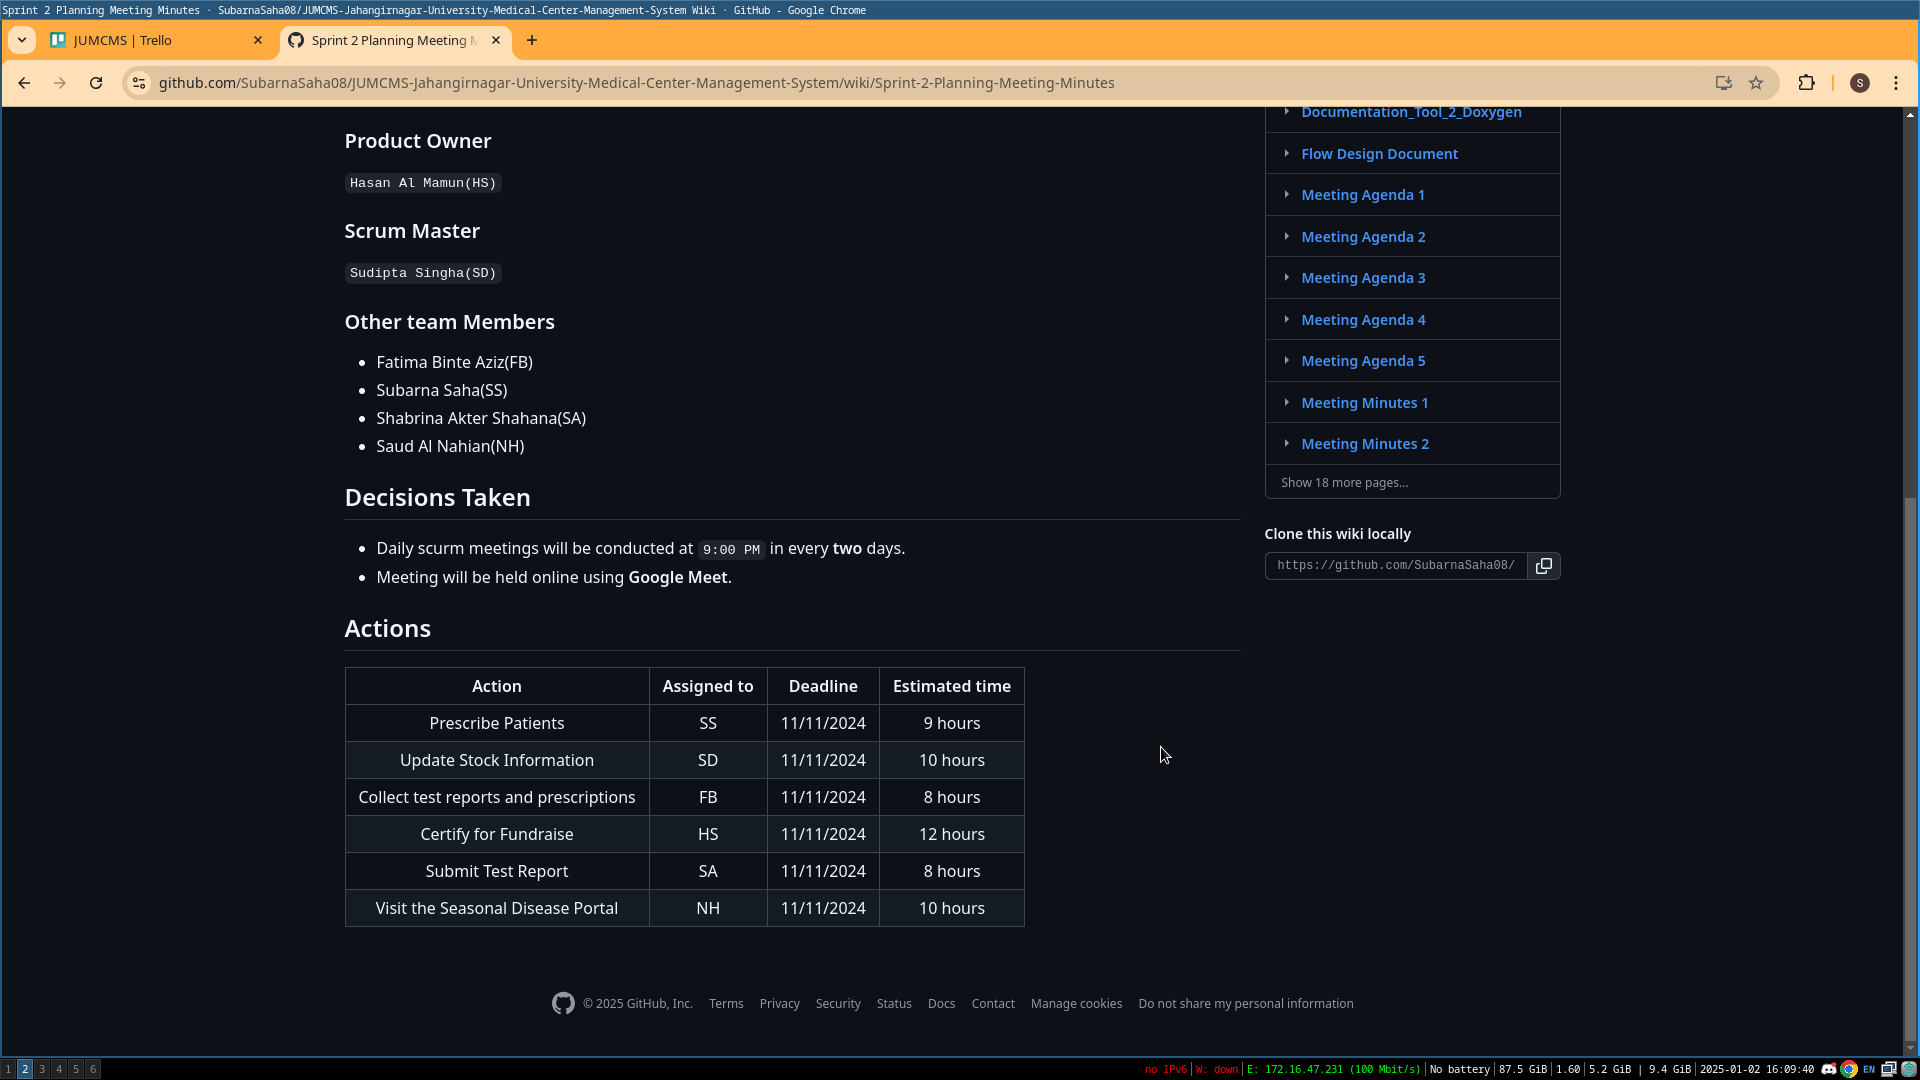
\includegraphics[width=1\textwidth]{images/spr2plan3.png}   
    \caption{Github wiki screenshot}
    \label{fig:spr2plan3}
\end{figure}
\newpage
\subsection{Scrum Meeting 1}
I was appointed the scrum master in this sprint. I arranged 4 scrum meeting during this sprint. In the first
scrum meeting my update are:
\begin{itemize}
    \item Yesterday: Created prototype UI for the "Update Stock Information".
    \item Today: Will prepare test cases for the controllers.
    \item Impediments: None.
\end{itemize}
\begin{figure}[H]
    \centering
    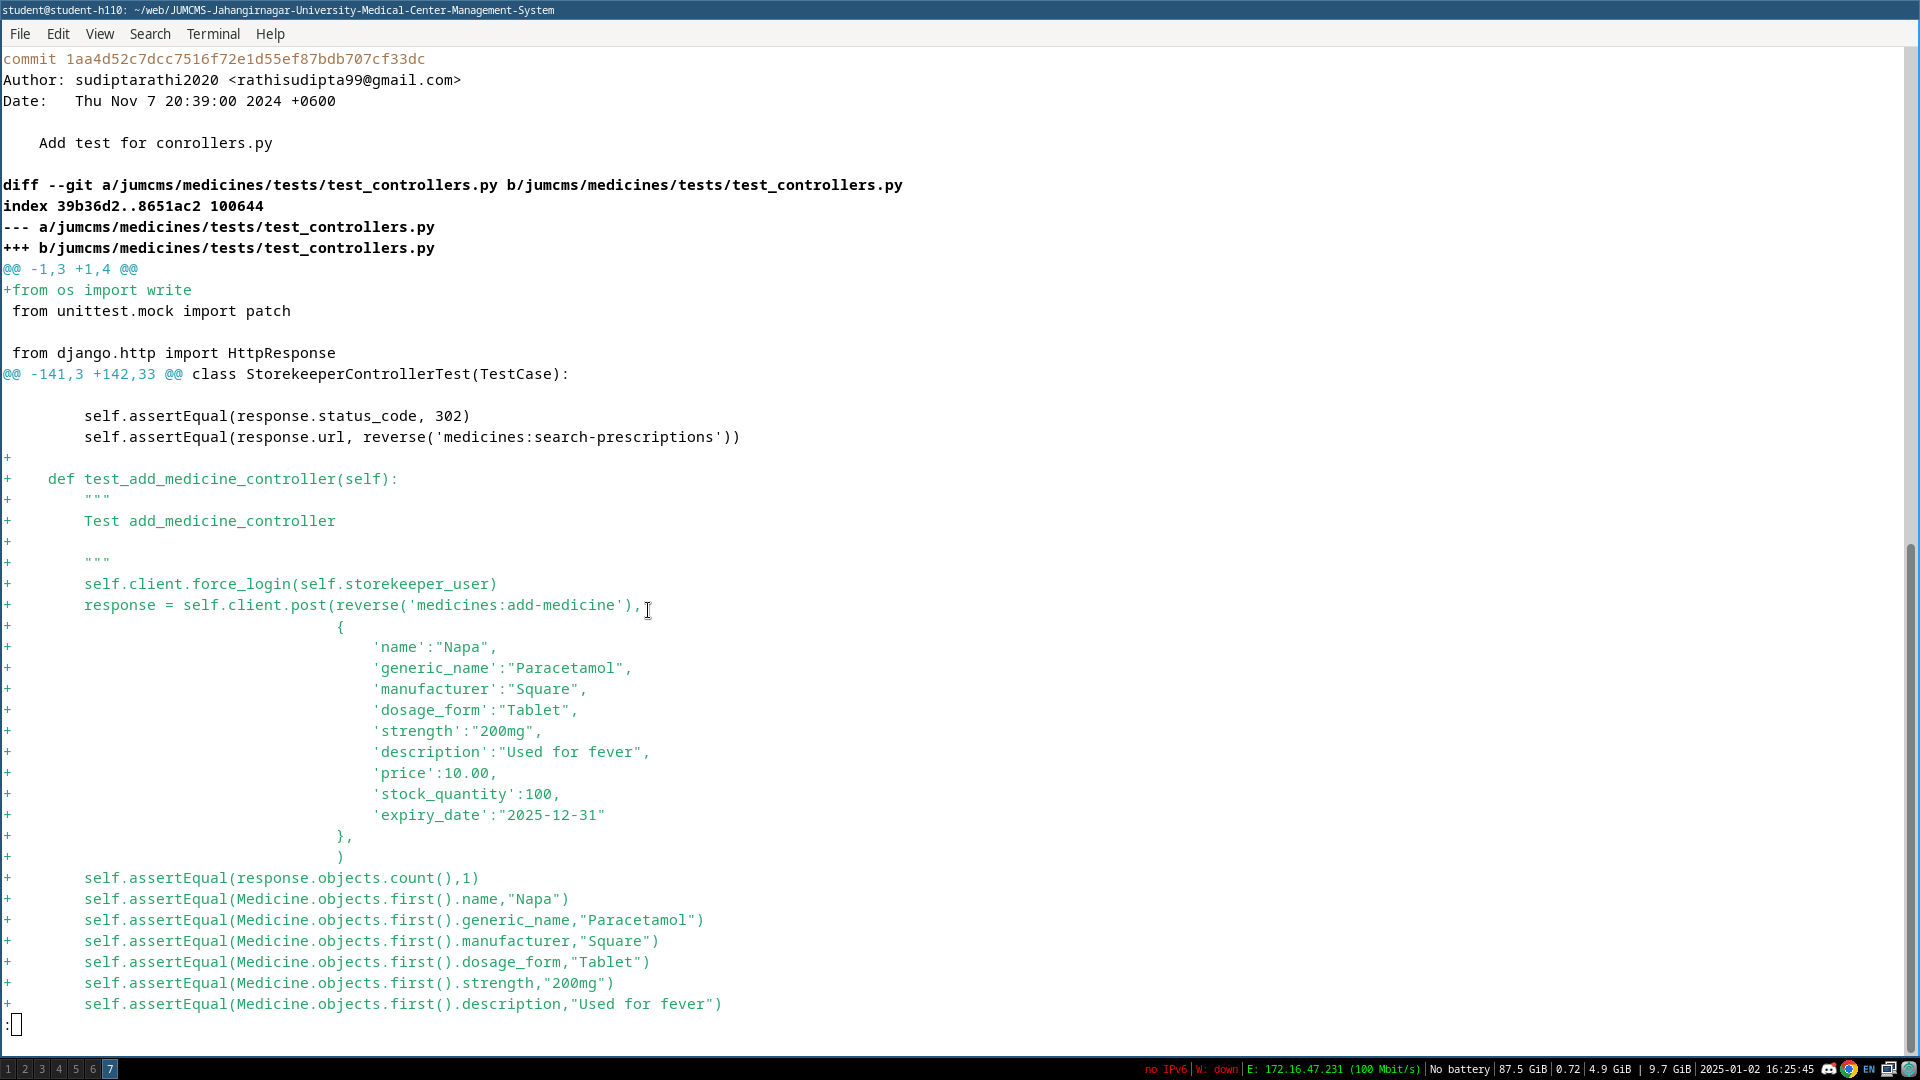
\includegraphics[width=1\textwidth]{images/meet11.png}   
    \caption{Git log of adding test case commit}
    \label{fig:meet11}
\end{figure}
\begin{figure}[H]
    \centering
    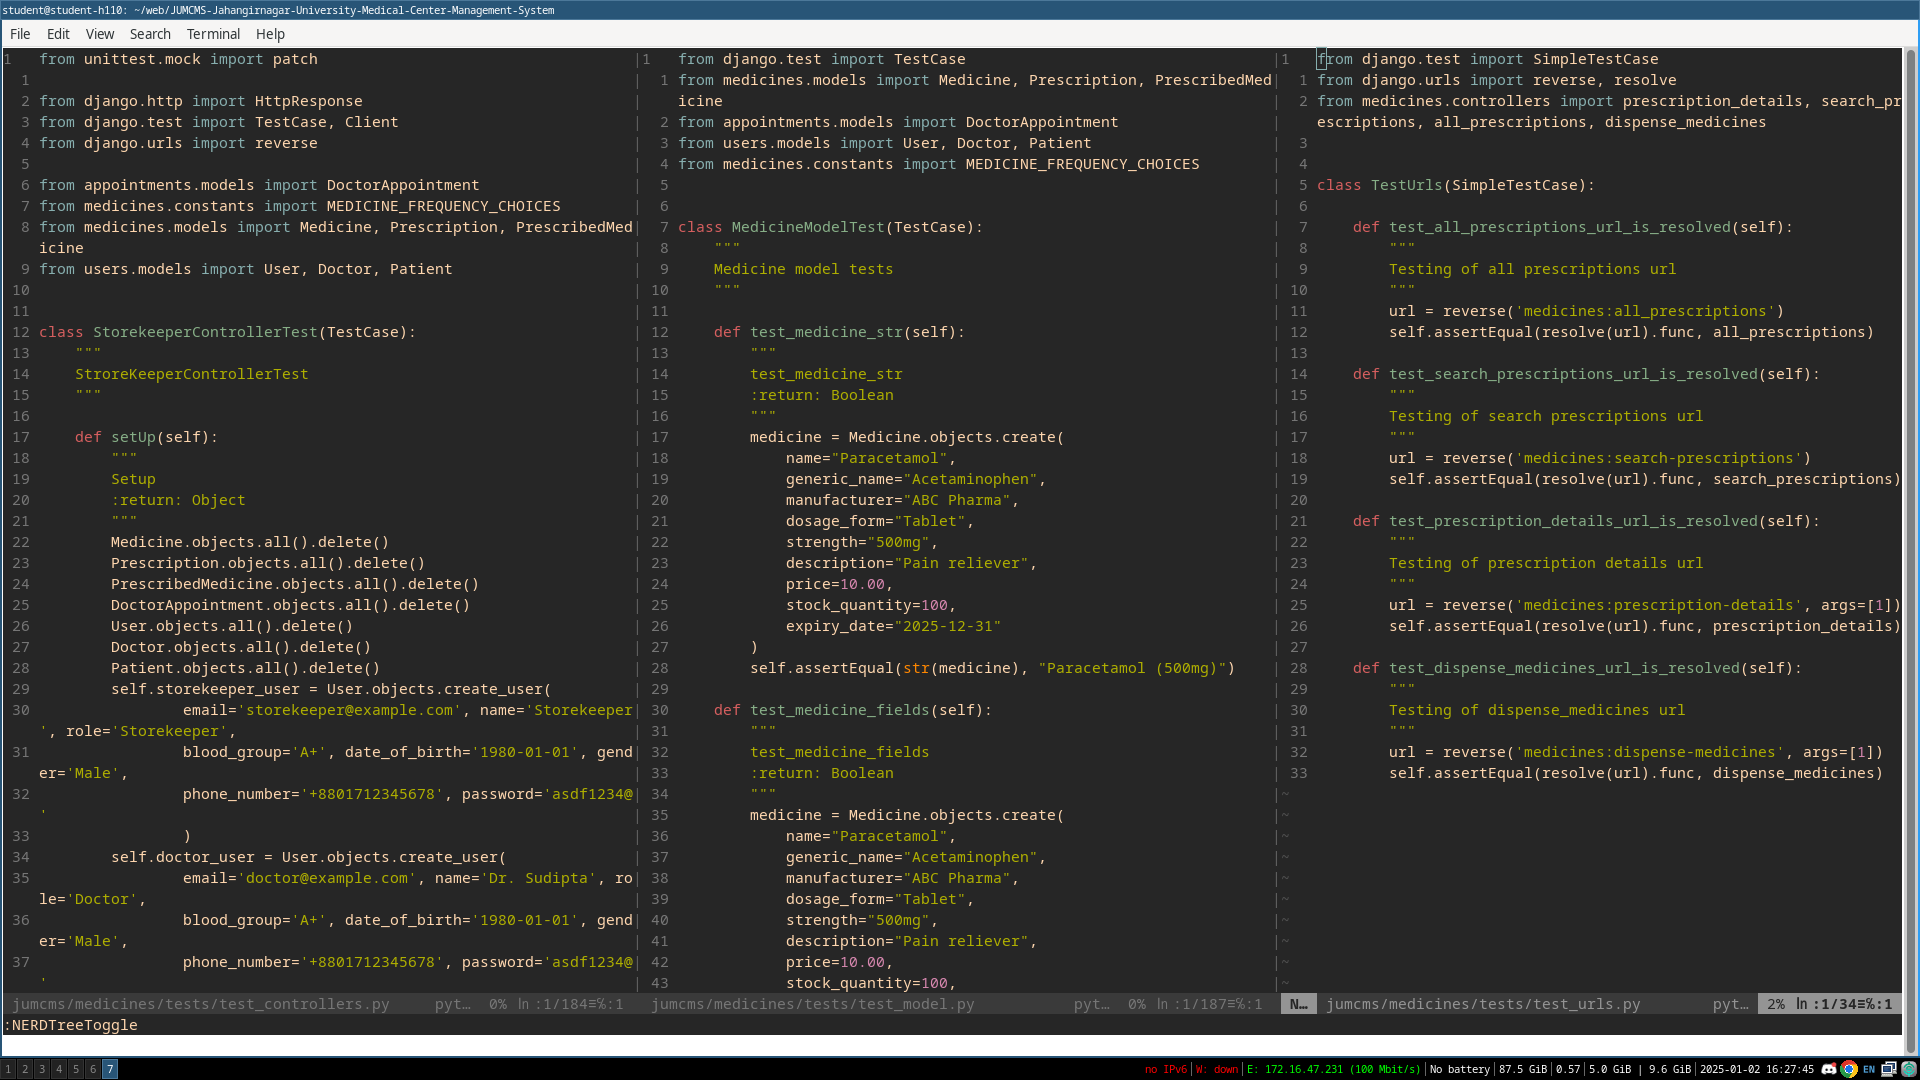
\includegraphics[width=1\textwidth]{images/meet12.png}   
    \caption{Example Test case for TDD Approach}
    \label{fig:meet12}
\end{figure}
\begin{figure}[H]
    \centering
    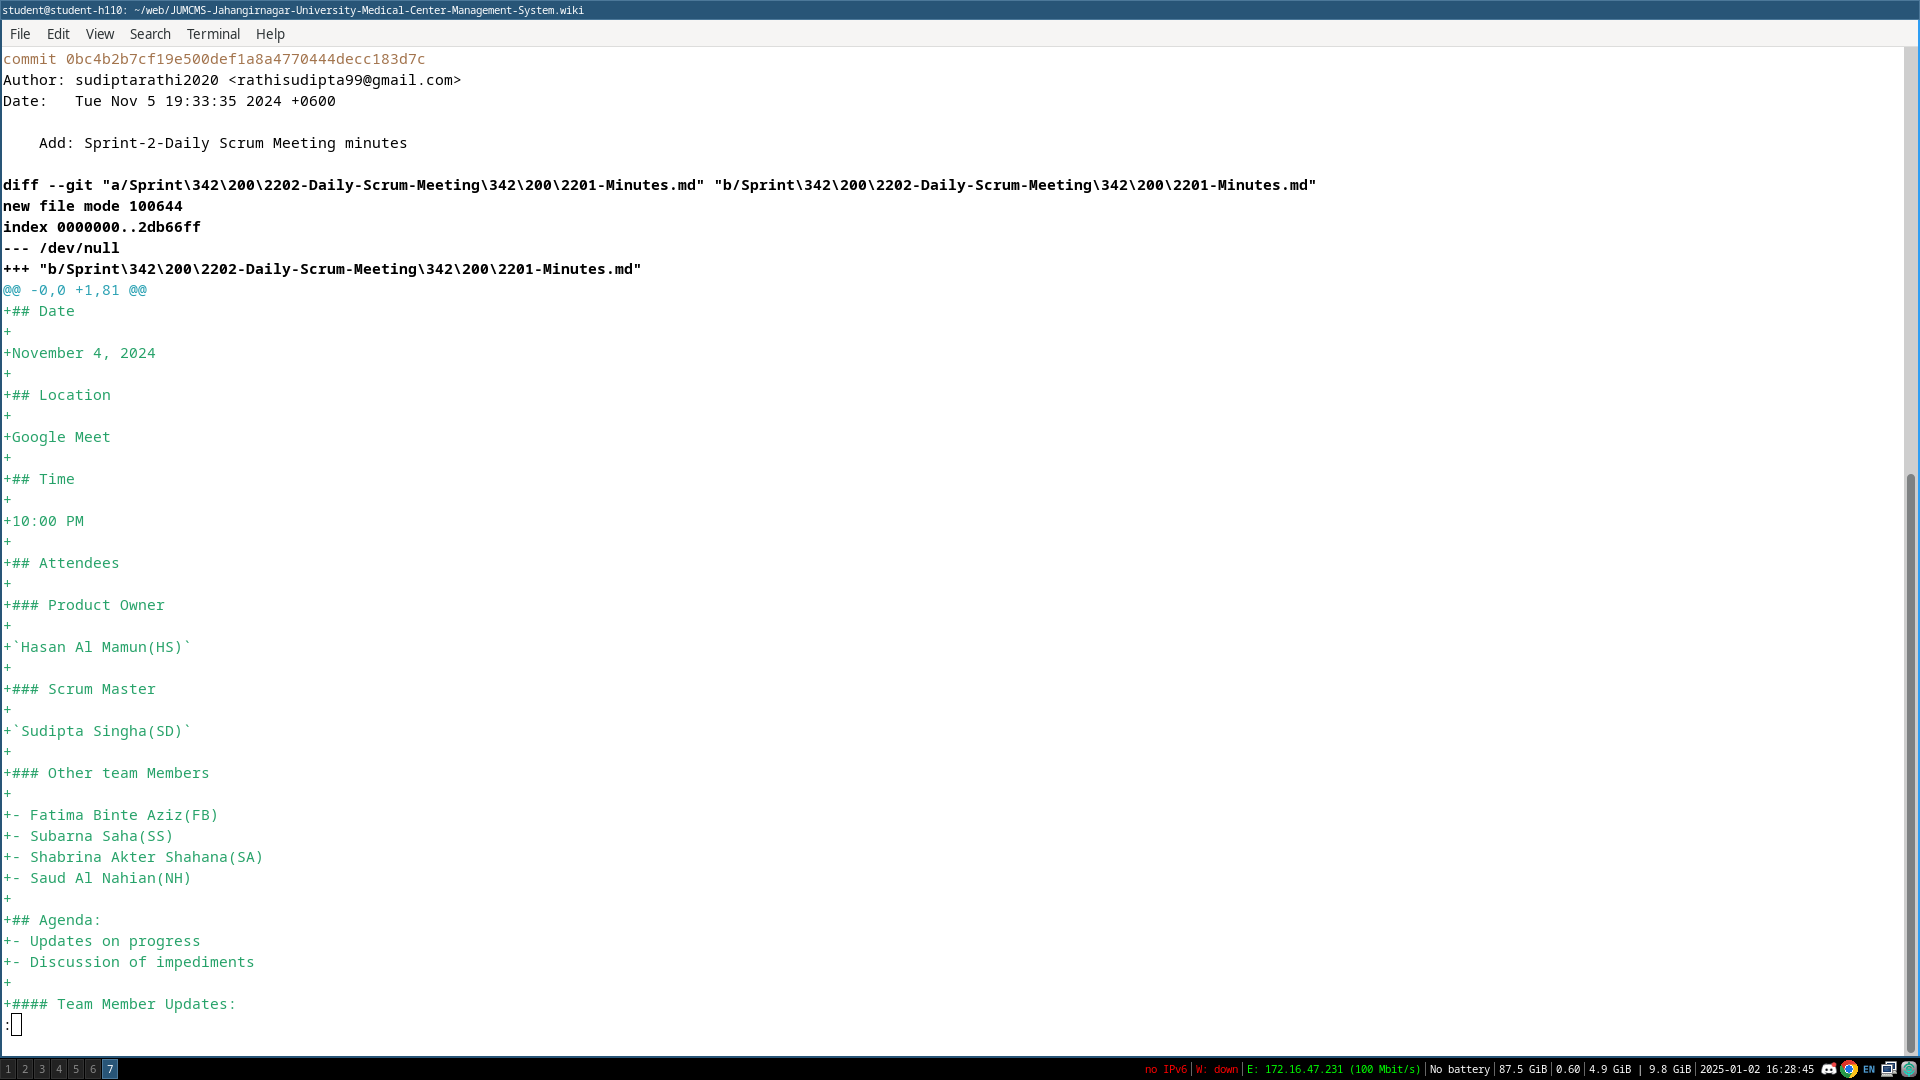
\includegraphics[width=1\textwidth]{images/meet13.png}   
    \caption{Gitlog for scrum 1 meeting minutes updated by me}
    \label{fig:meet13}
\end{figure}

\newpage
\subsection{Scrum Meeting 2 and 3}
\begin{itemize}
    \item Yesterday: Created prototype UI for the "Update Stock Information".
    \item Today: Created test cases and implemented some portion of the UI.
    \item Impediments: None.
\end{itemize}
\begin{figure}[H]
    \centering
    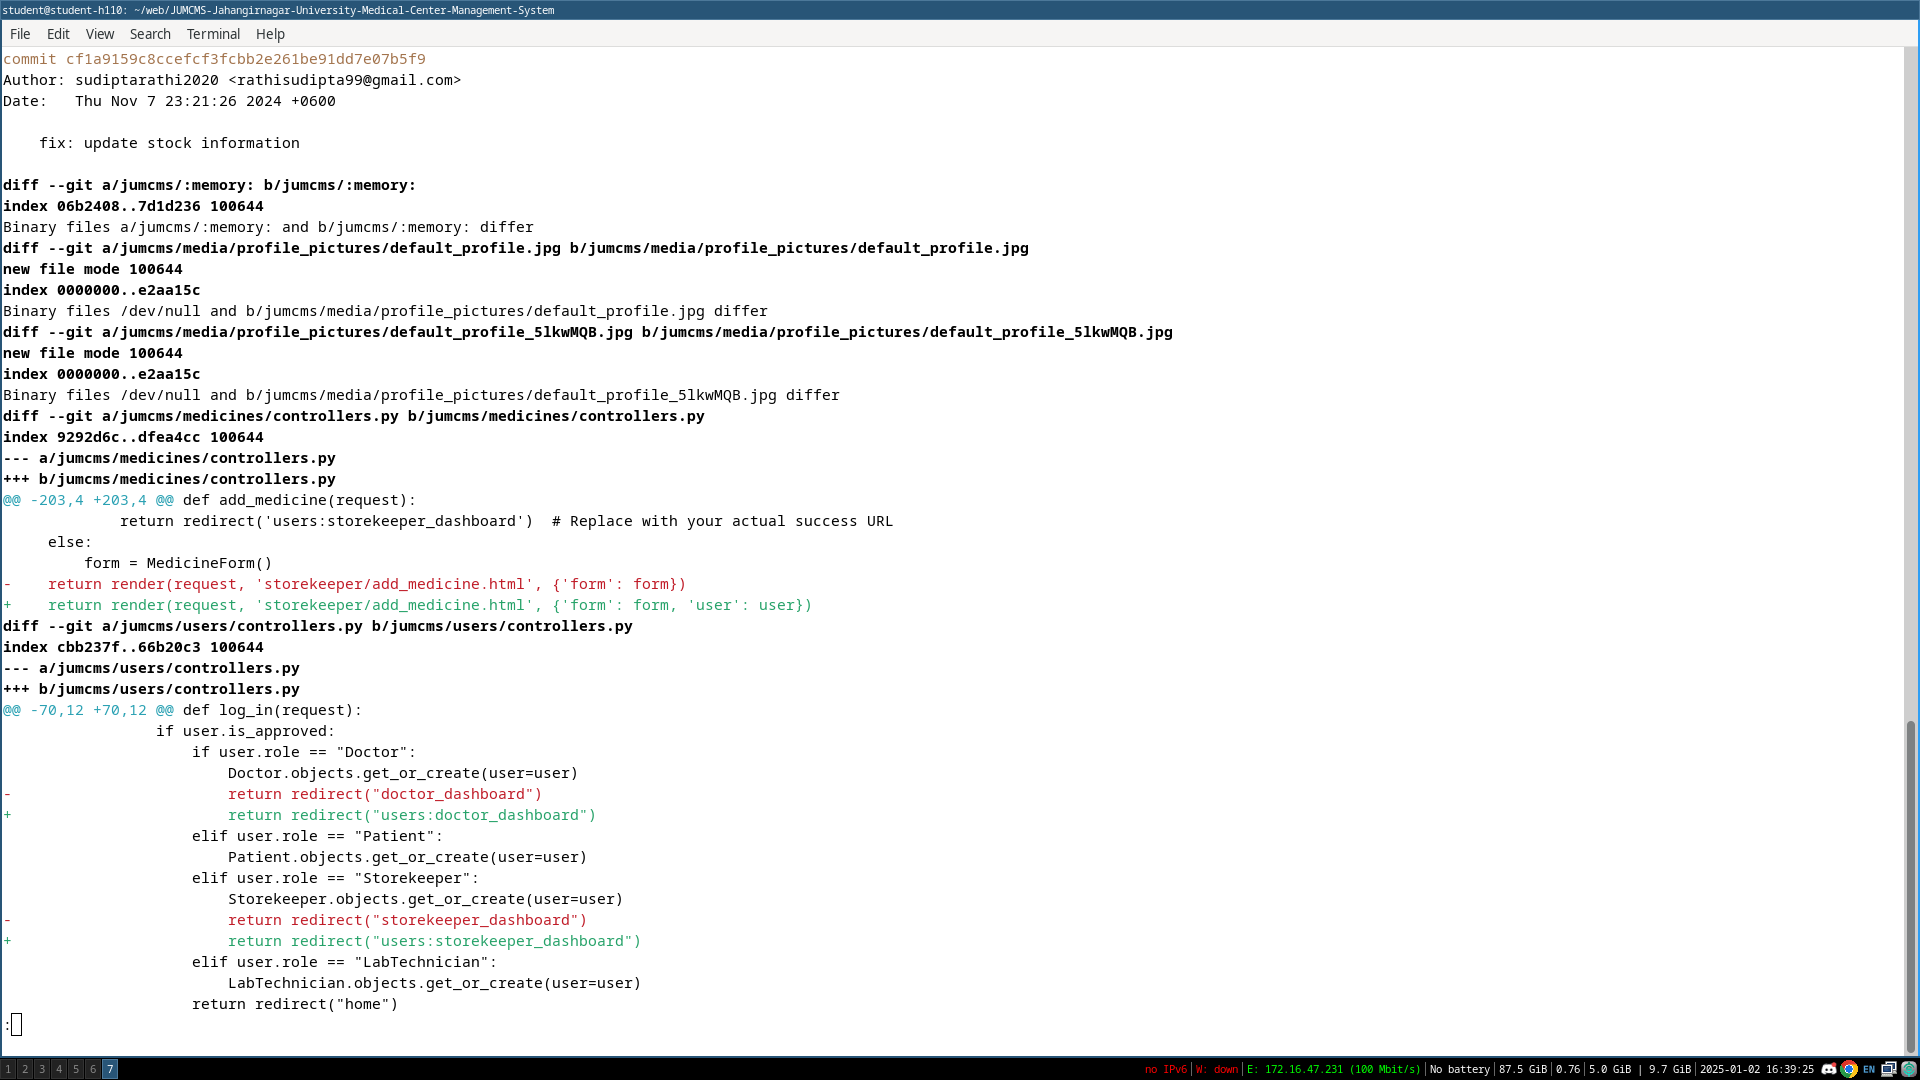
\includegraphics[width=1\textwidth]{images/meet21.png}   
    \caption{Git log for update stock information}
    \label{fig:meet21}
\end{figure}
\begin{figure}[H]
    \centering
    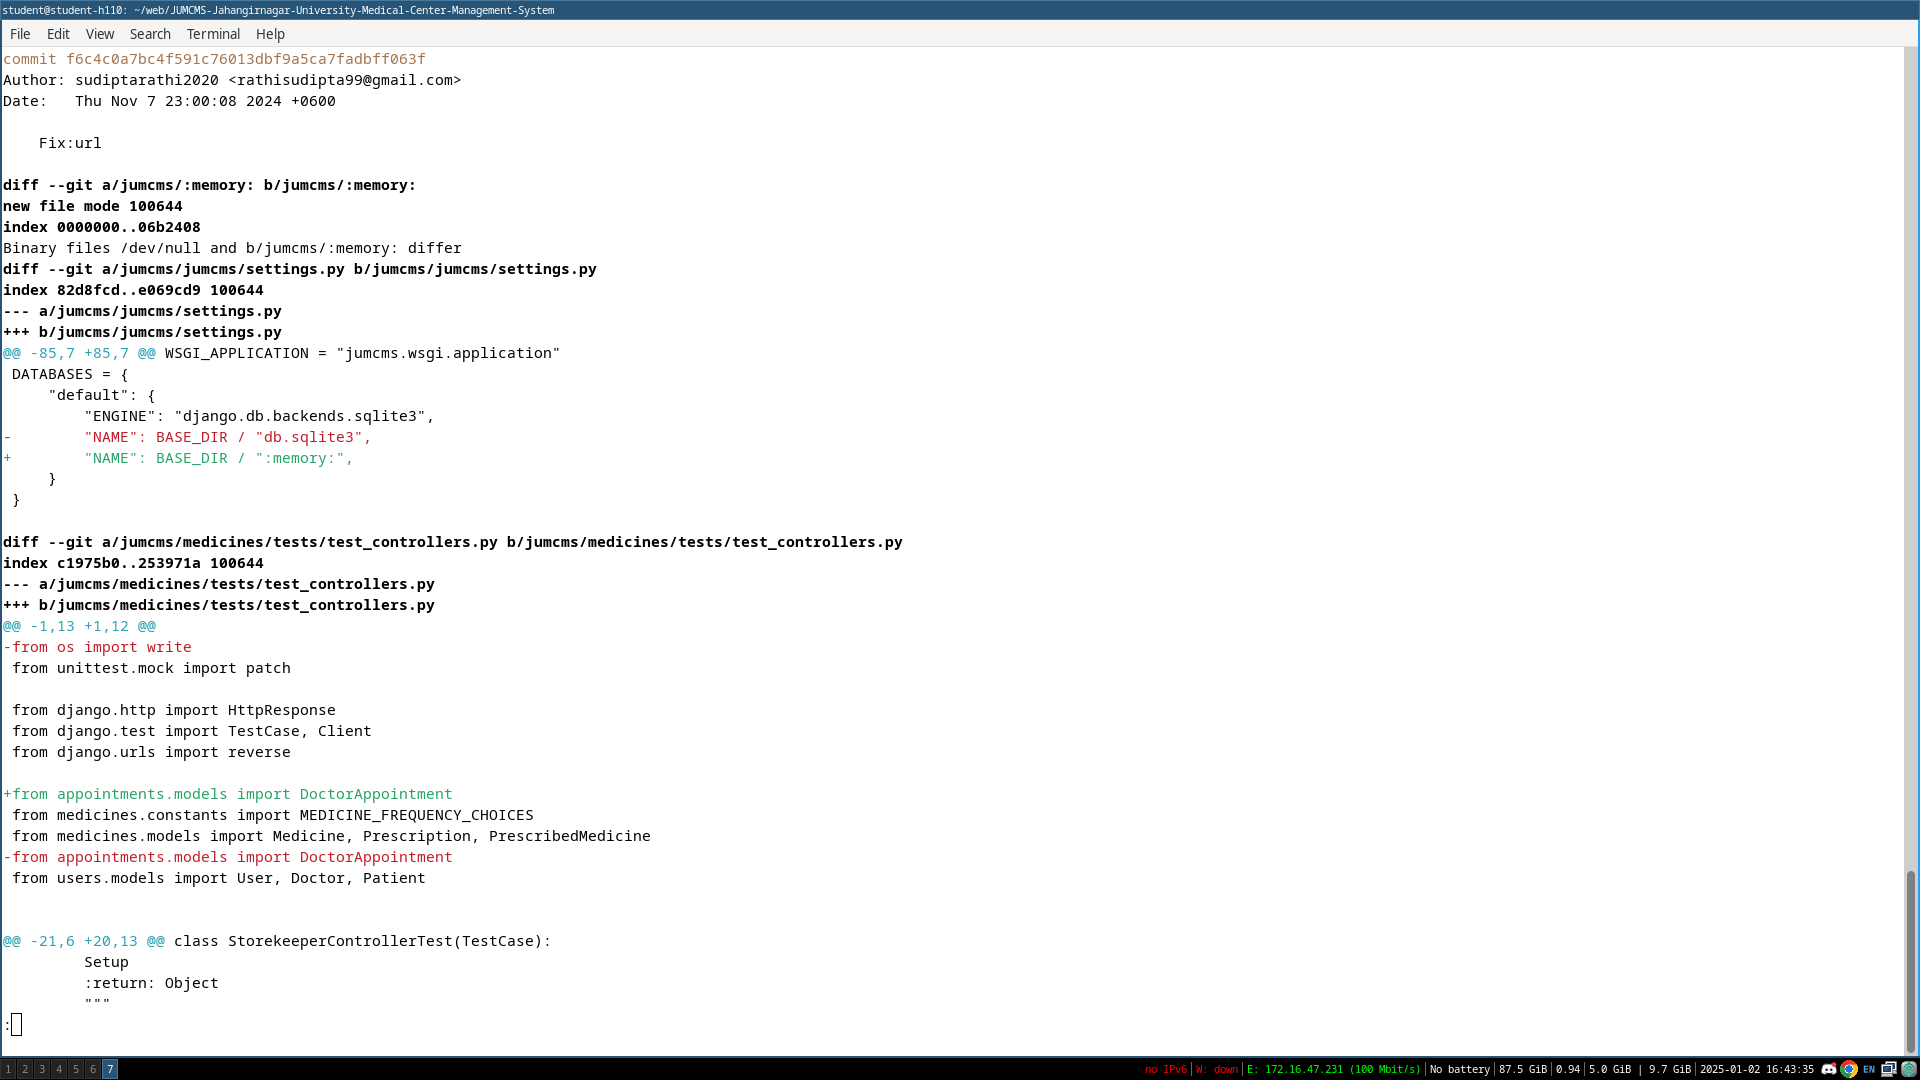
\includegraphics[width=1\textwidth]{images/meet22.png}   
    \caption{Git log of fixing url}
    \label{fig:meet22}
\end{figure}
\begin{figure}[H]
    \centering
    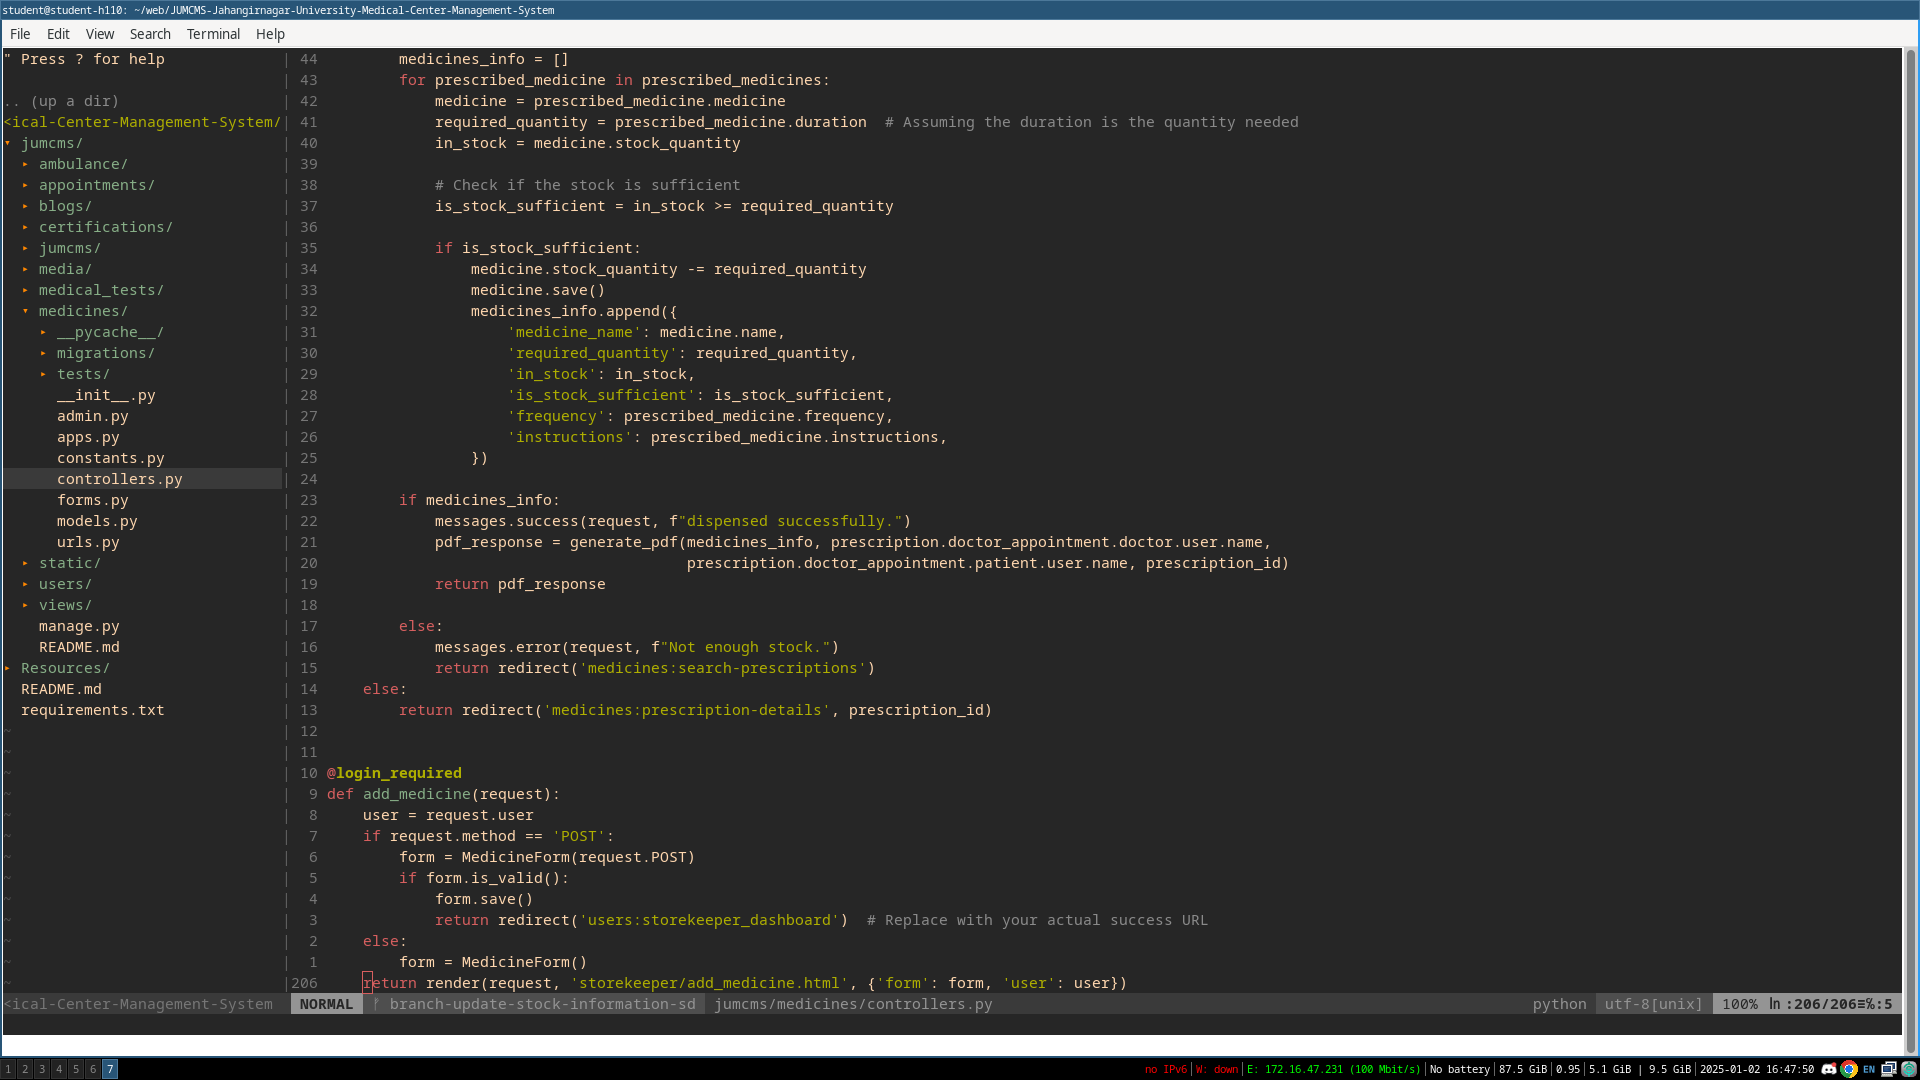
\includegraphics[width=1\textwidth]{images/meet201.png}   
    \caption{Example Controllers code}
    \label{fig:meet201}
\end{figure}

\begin{figure}[H]
    \centering
    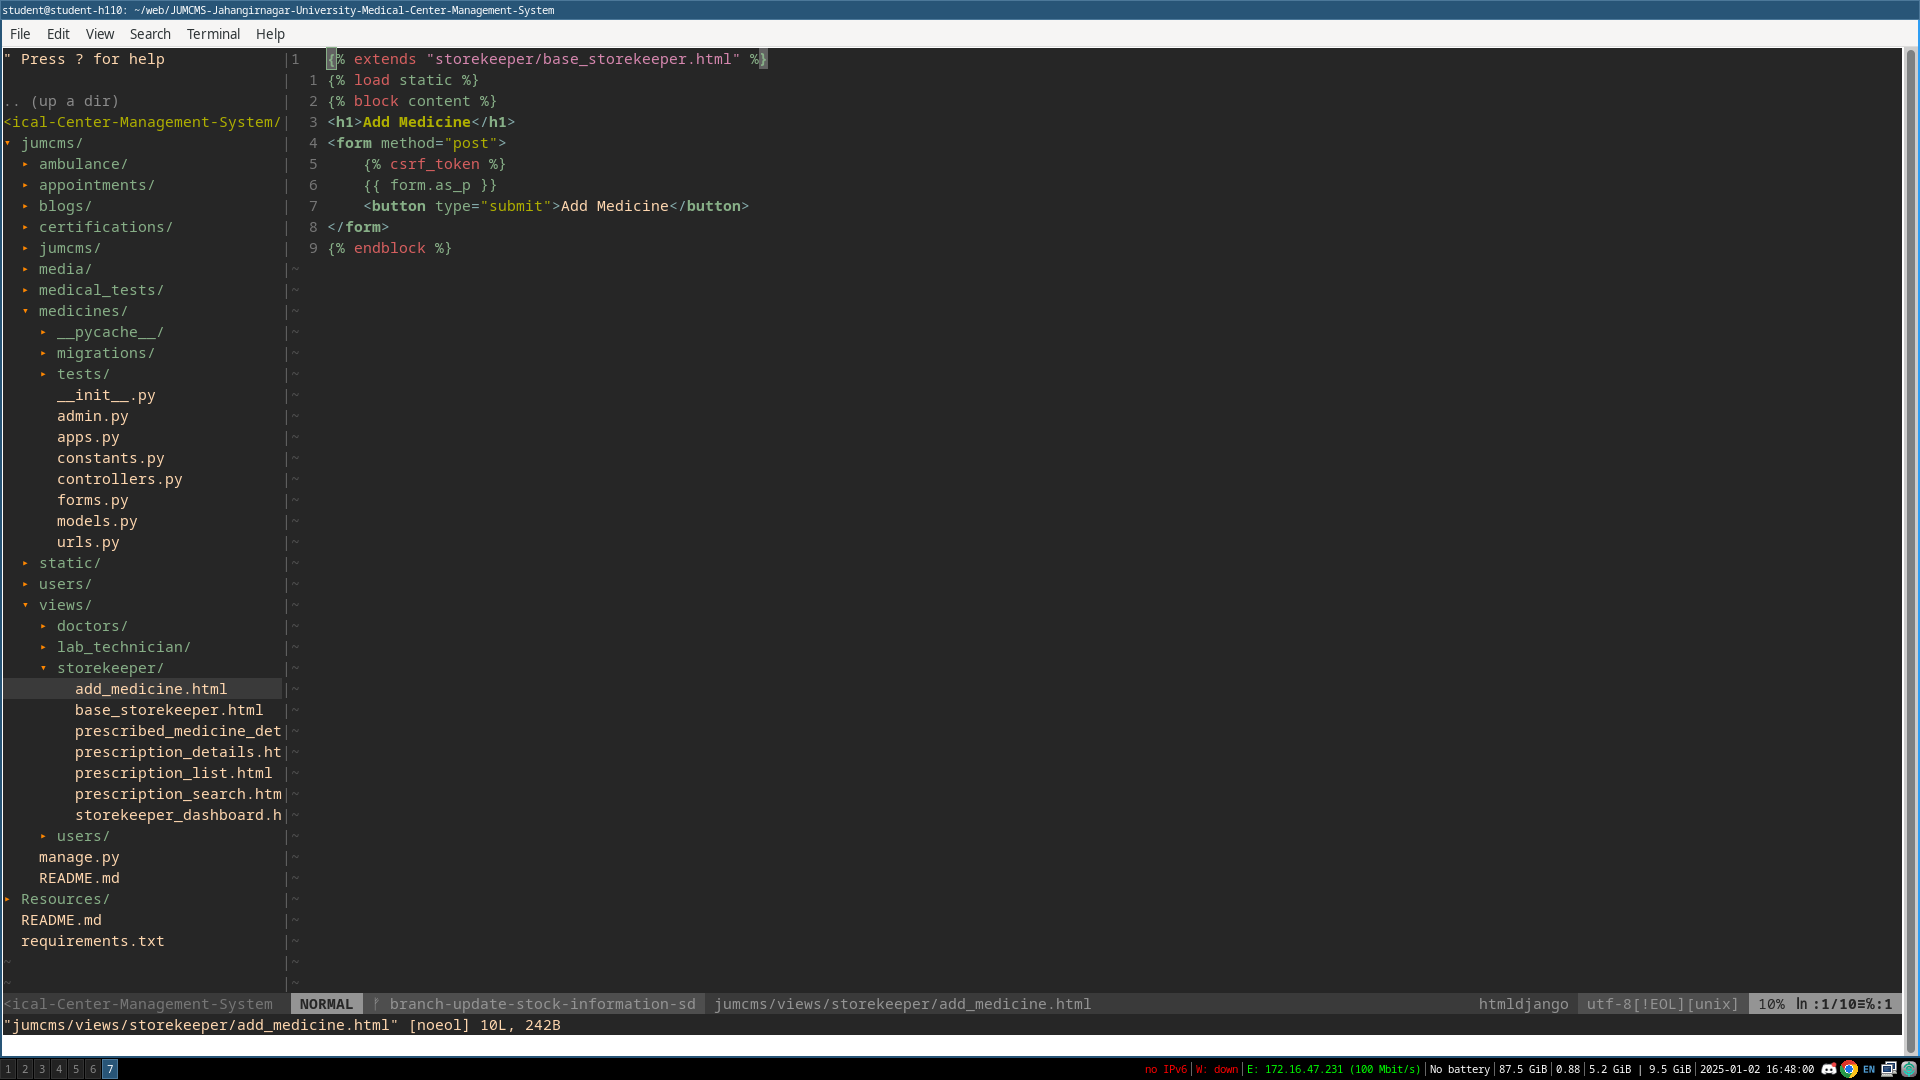
\includegraphics[width=1\textwidth]{images/meet202.png}   
    \caption{Example UI Code}
    \label{fig:meet202}
\end{figure}
\begin{figure}[H]
    \centering
    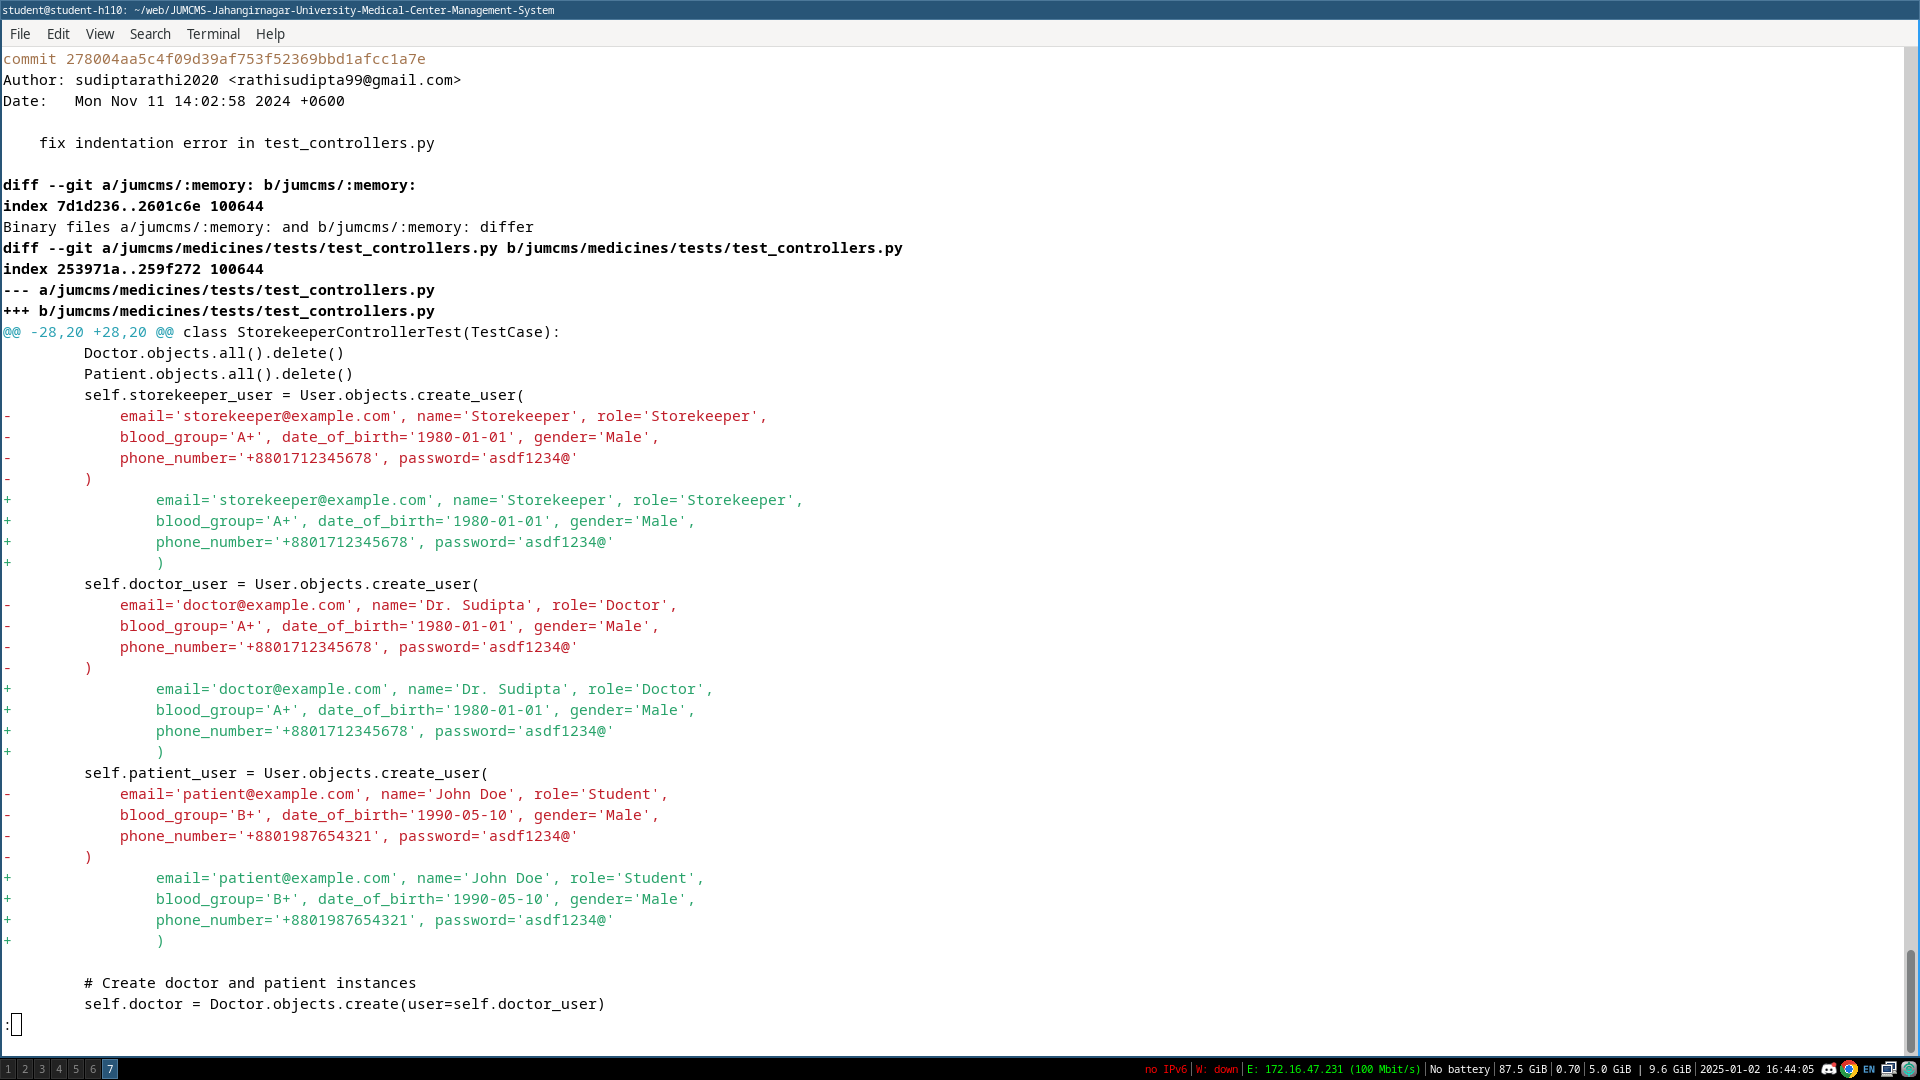
\includegraphics[width=1\textwidth]{images/meet31.png}   
    \caption{Git log}
    \label{fig:meet31}
\end{figure}
\begin{figure}[H]
    \centering
    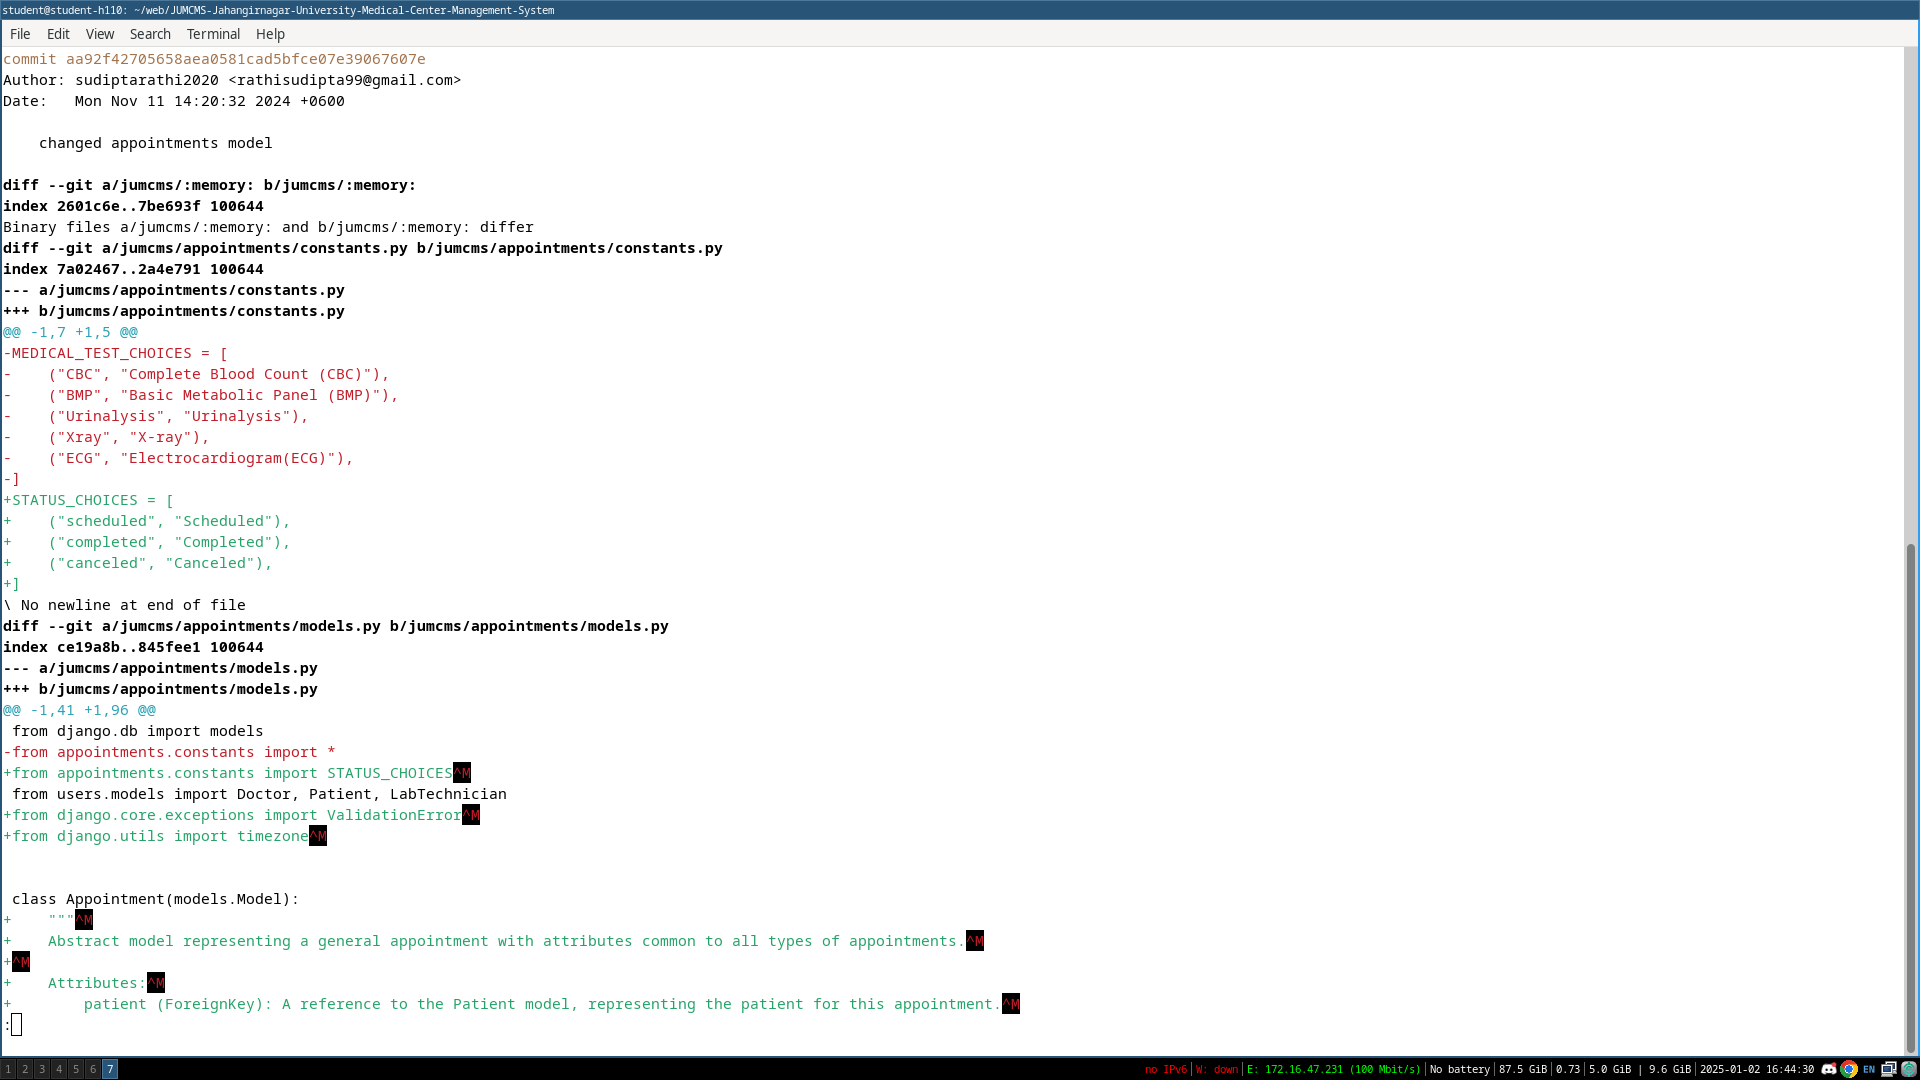
\includegraphics[width=1\textwidth]{images/meet32.png}   
    \caption{Git log}
    \label{fig:meet32}
\end{figure}
\begin{figure}[H]
    \centering
    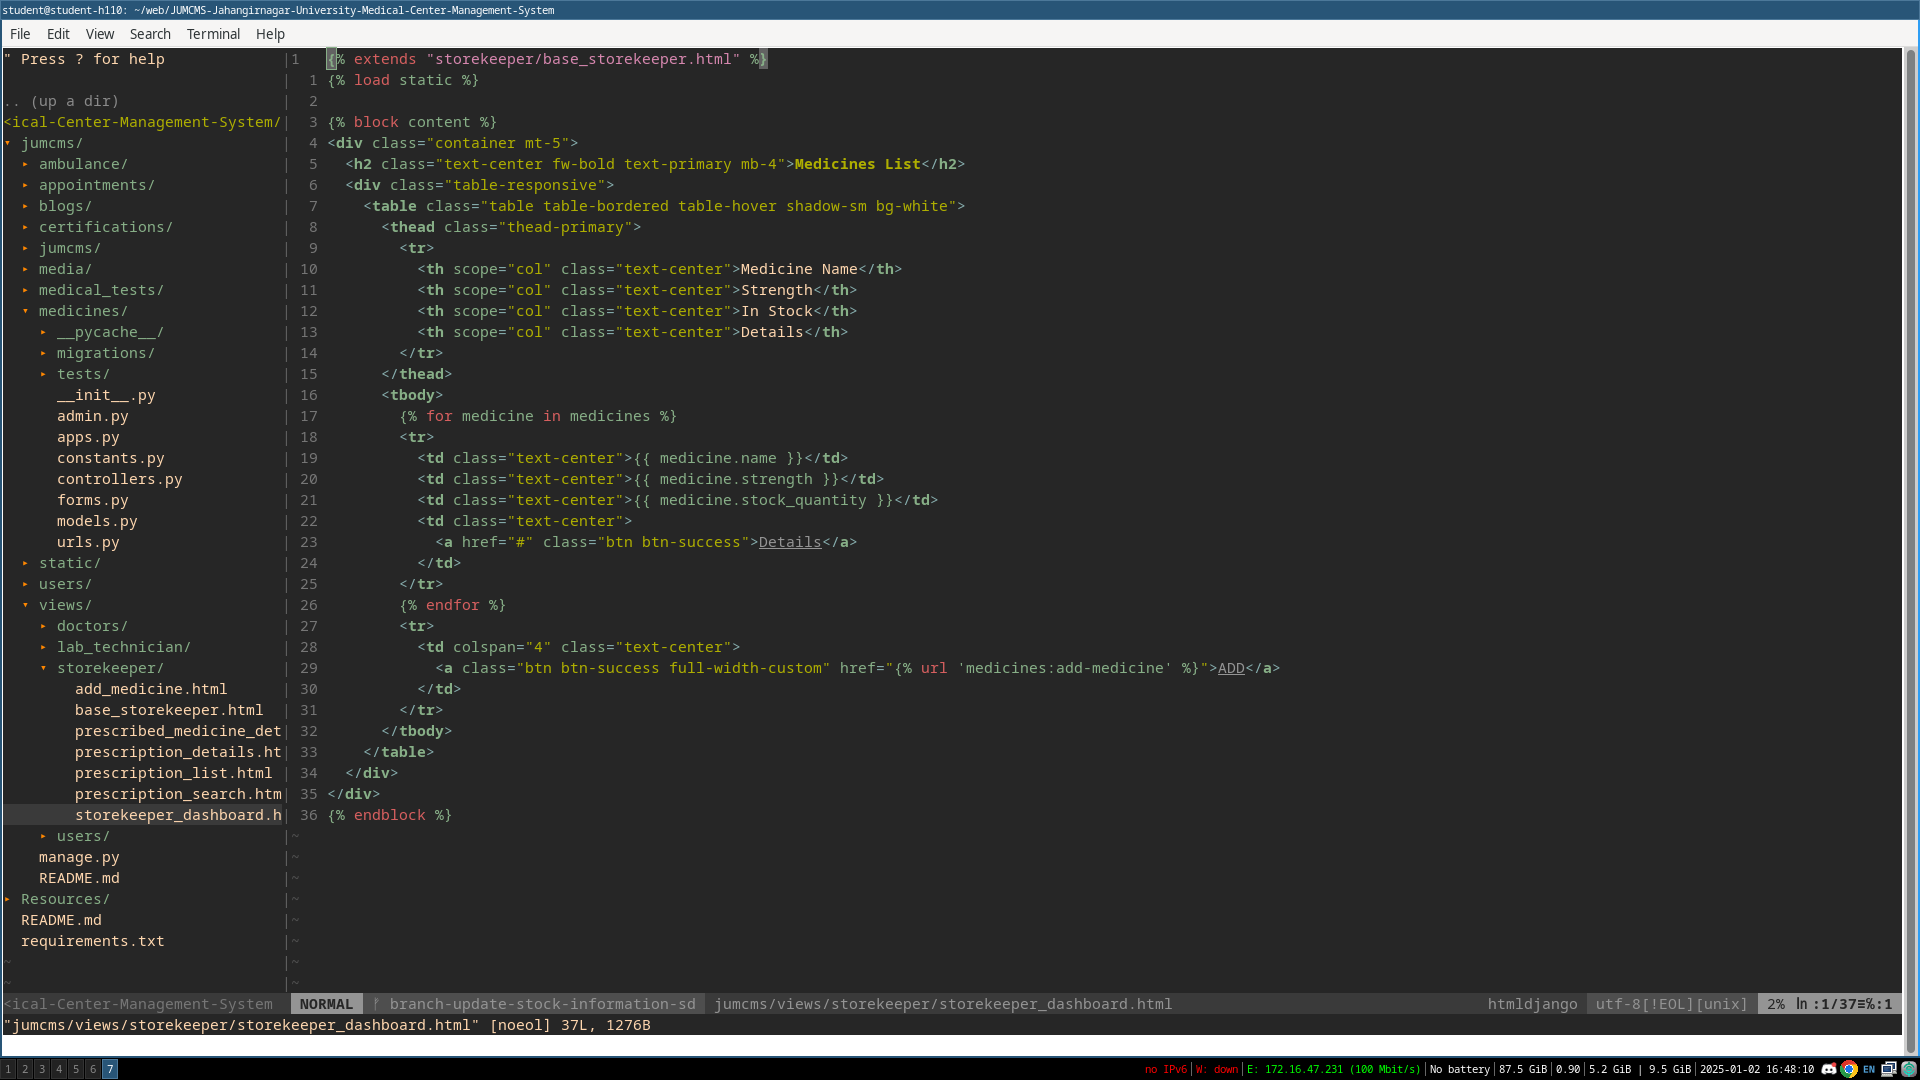
\includegraphics[width=1\textwidth]{images/meet33.png}   
    \caption{Update Stock information}
    \label{fig:meet33}
\end{figure}


\newpage
\subsection{Scrum Meeting 4}
\begin{itemize}
    \item Yesterday: Implemented and Tested code according to test cases.
    \item Today: Merging, Pull Request, and Continuous Integration.
    \item Impediments: None.
\end{itemize}
\begin{figure}[H]
    \centering
    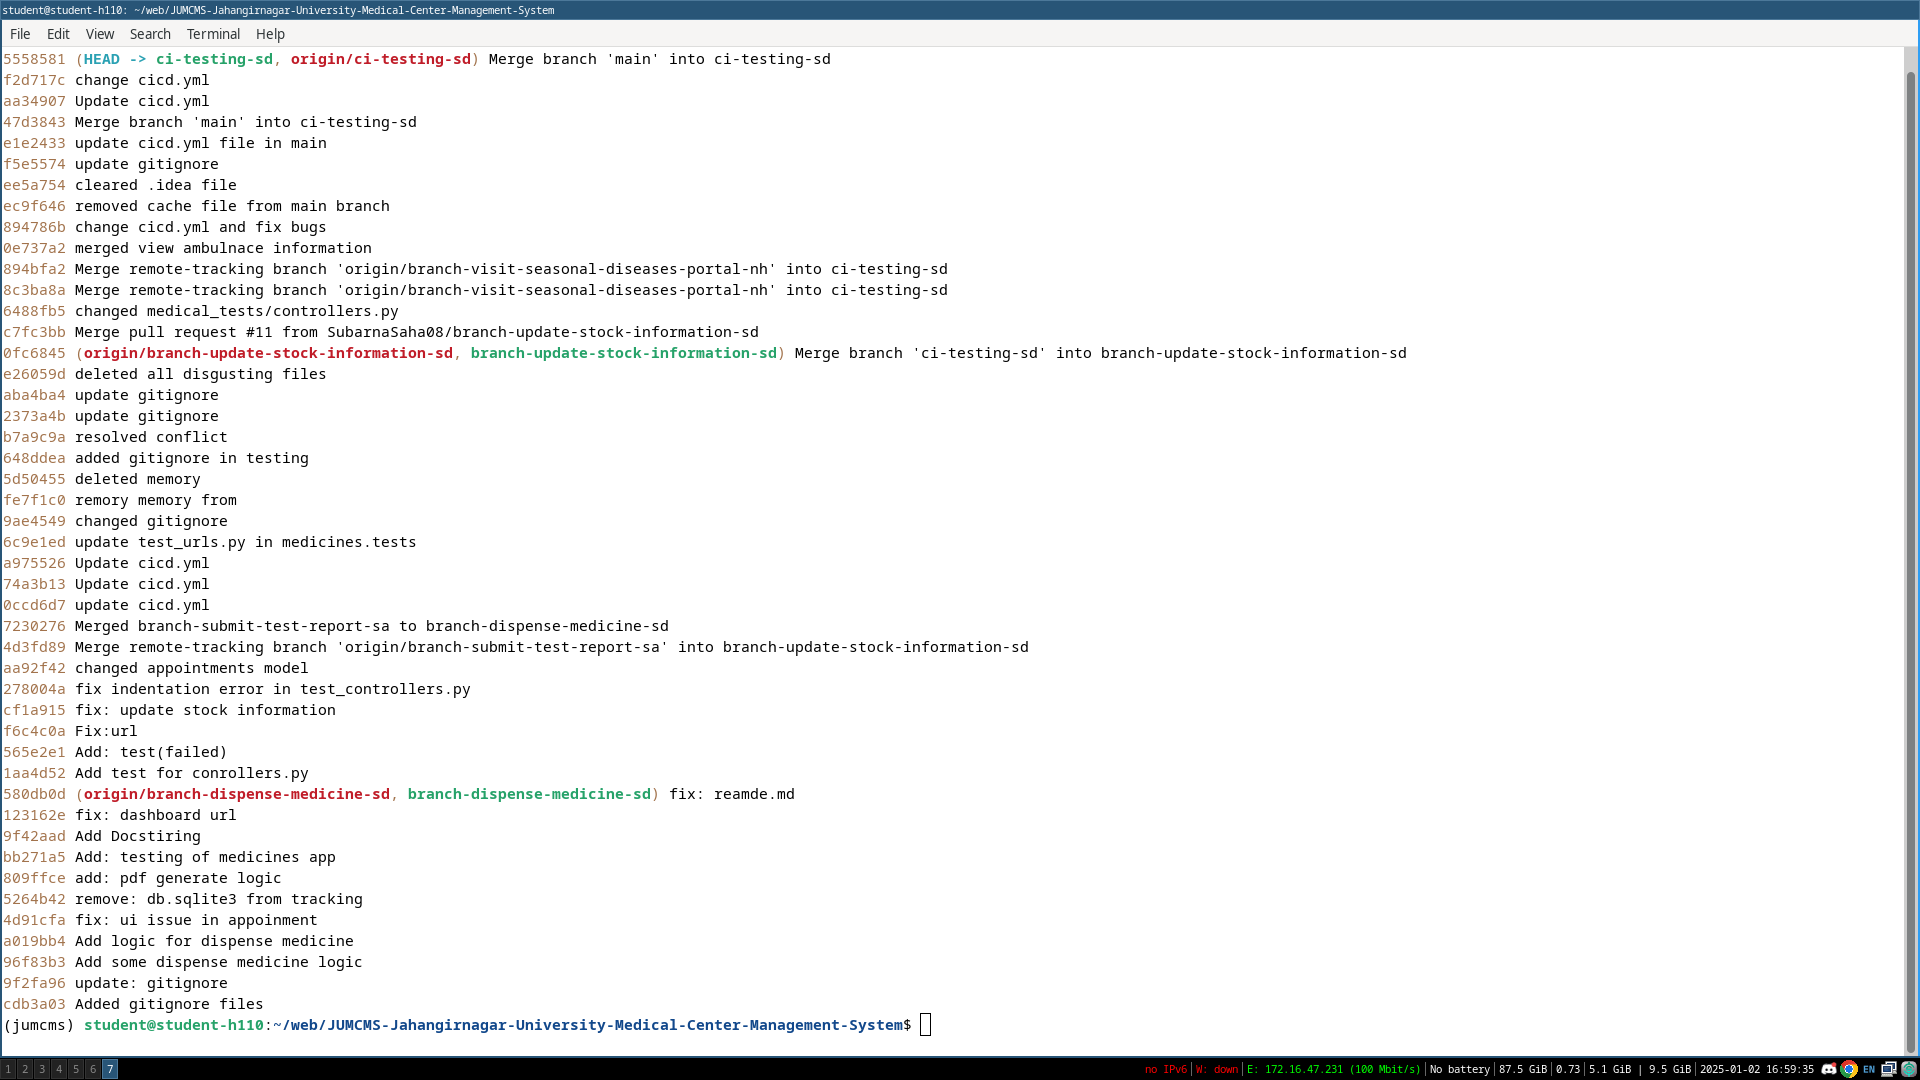
\includegraphics[width=1\textwidth]{images/meet41.png}
    \caption{git log}
    \label{fig:meet41}
\end{figure}

\begin{figure}[H]
    \centering
    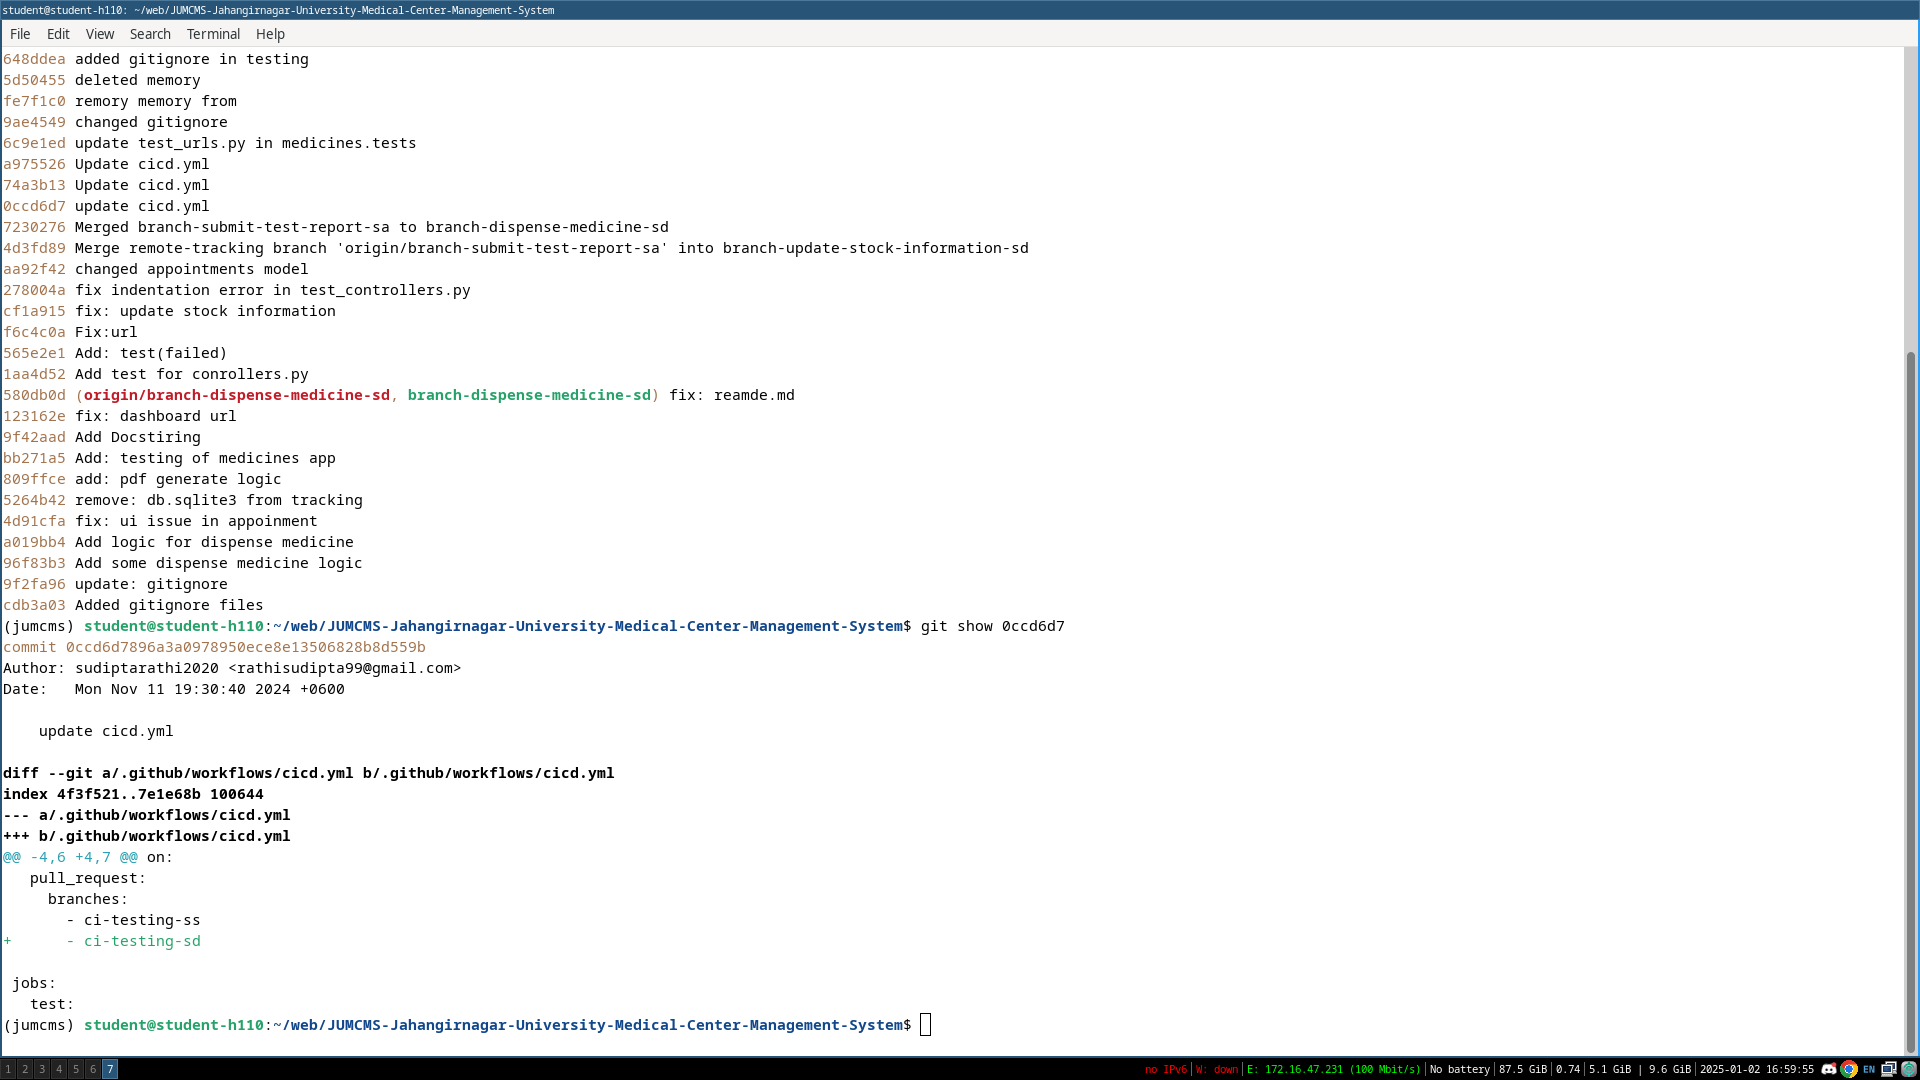
\includegraphics[width=1\textwidth]{images/meet42.png}
    \caption{git log}
    \label{fig:meet42}
\end{figure}


\begin{figure}[H]
    \centering
    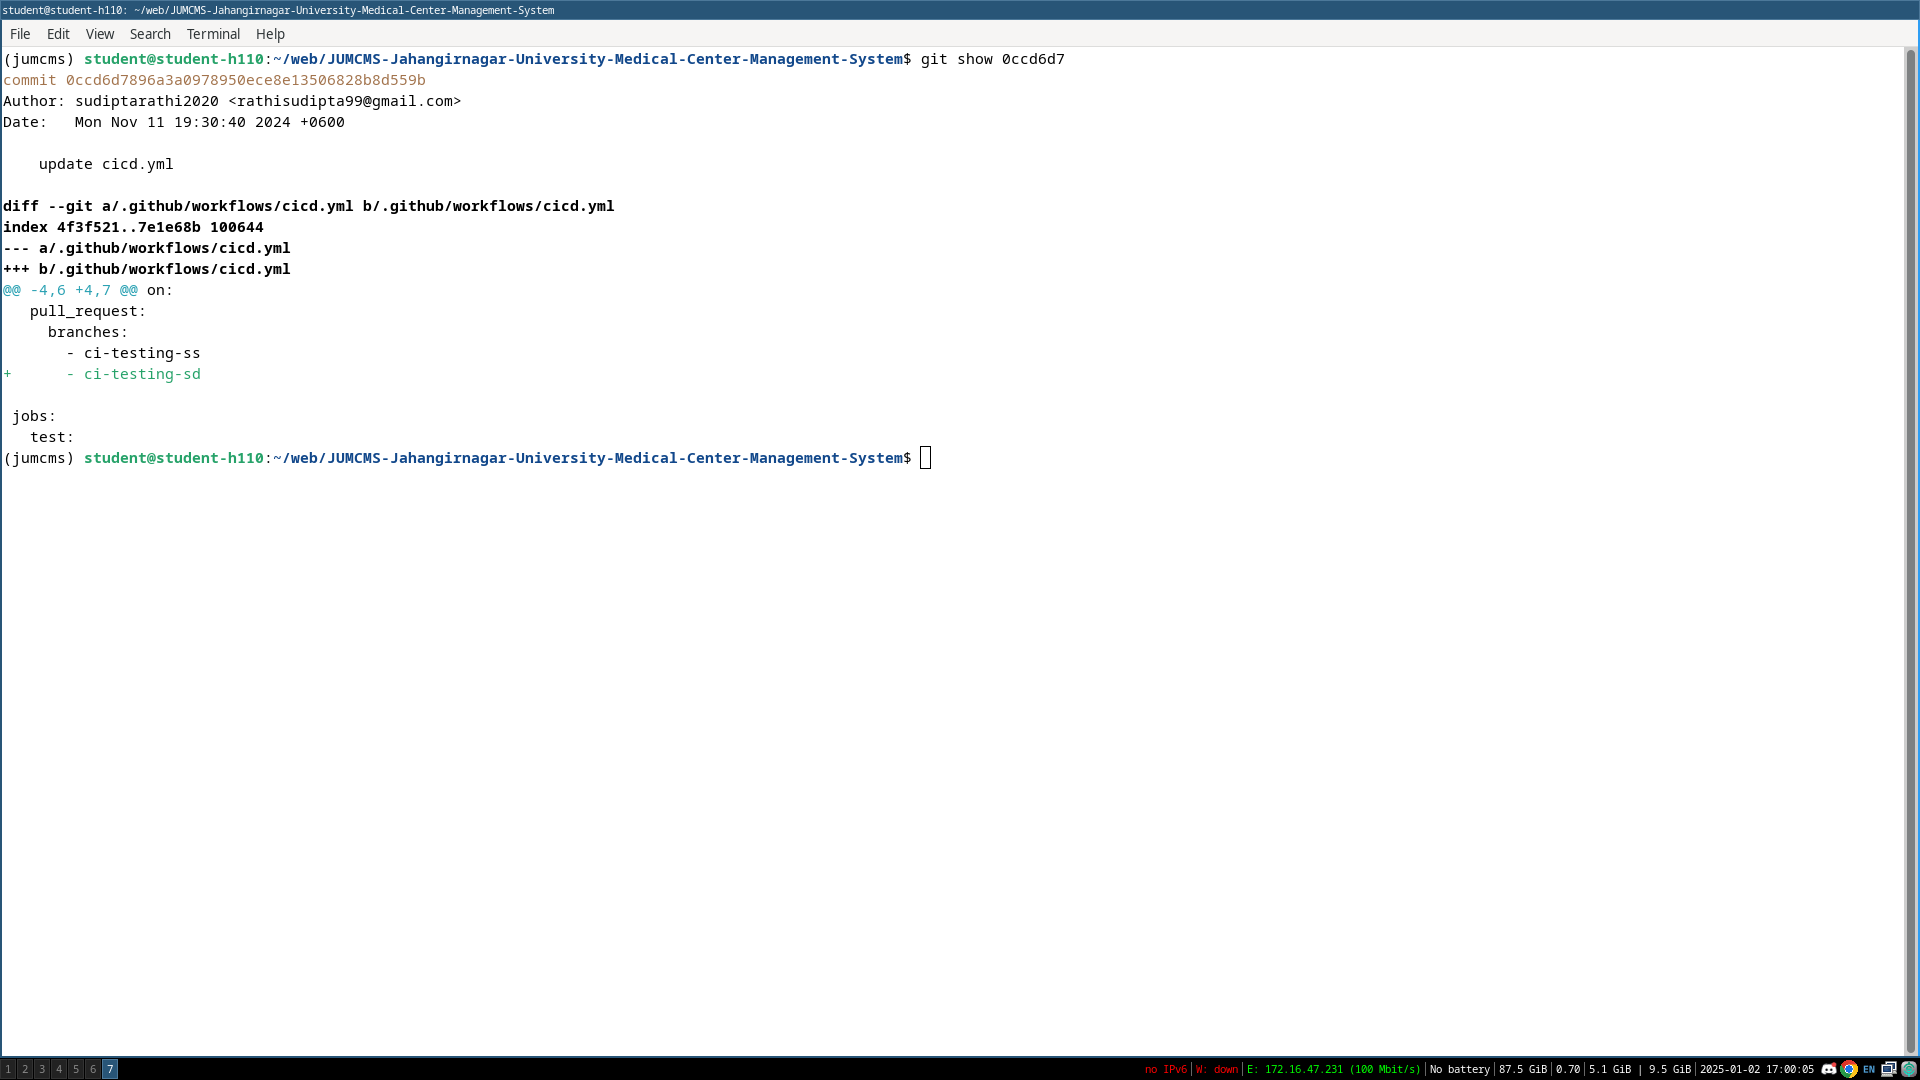
\includegraphics[width=1\textwidth]{images/meet43.png}
    \caption{git log}
    \label{fig:meet43}
\end{figure}

\begin{figure}[H]
    \centering
    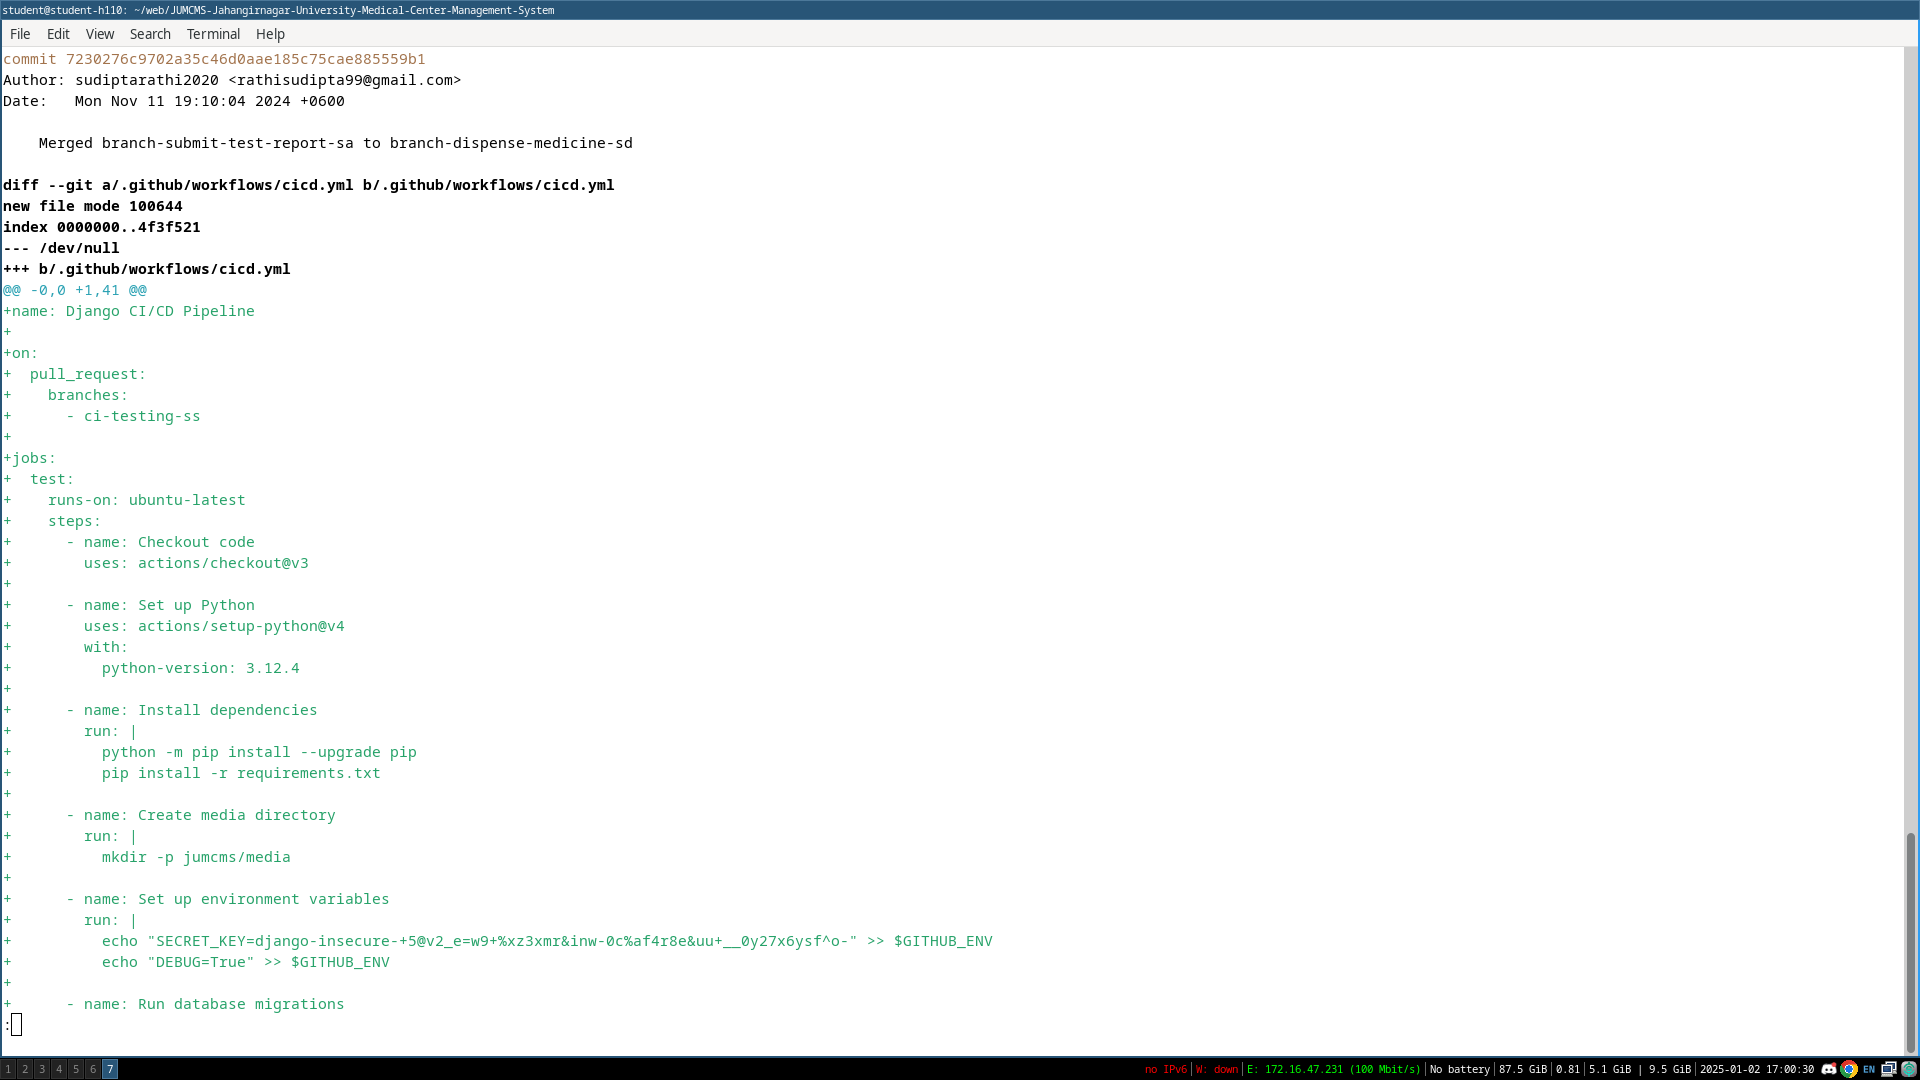
\includegraphics[width=1\textwidth]{images/meet44.png}
    \caption{git log}
    \label{fig:meet44}
\end{figure}

\begin{figure}[H]
    \centering
    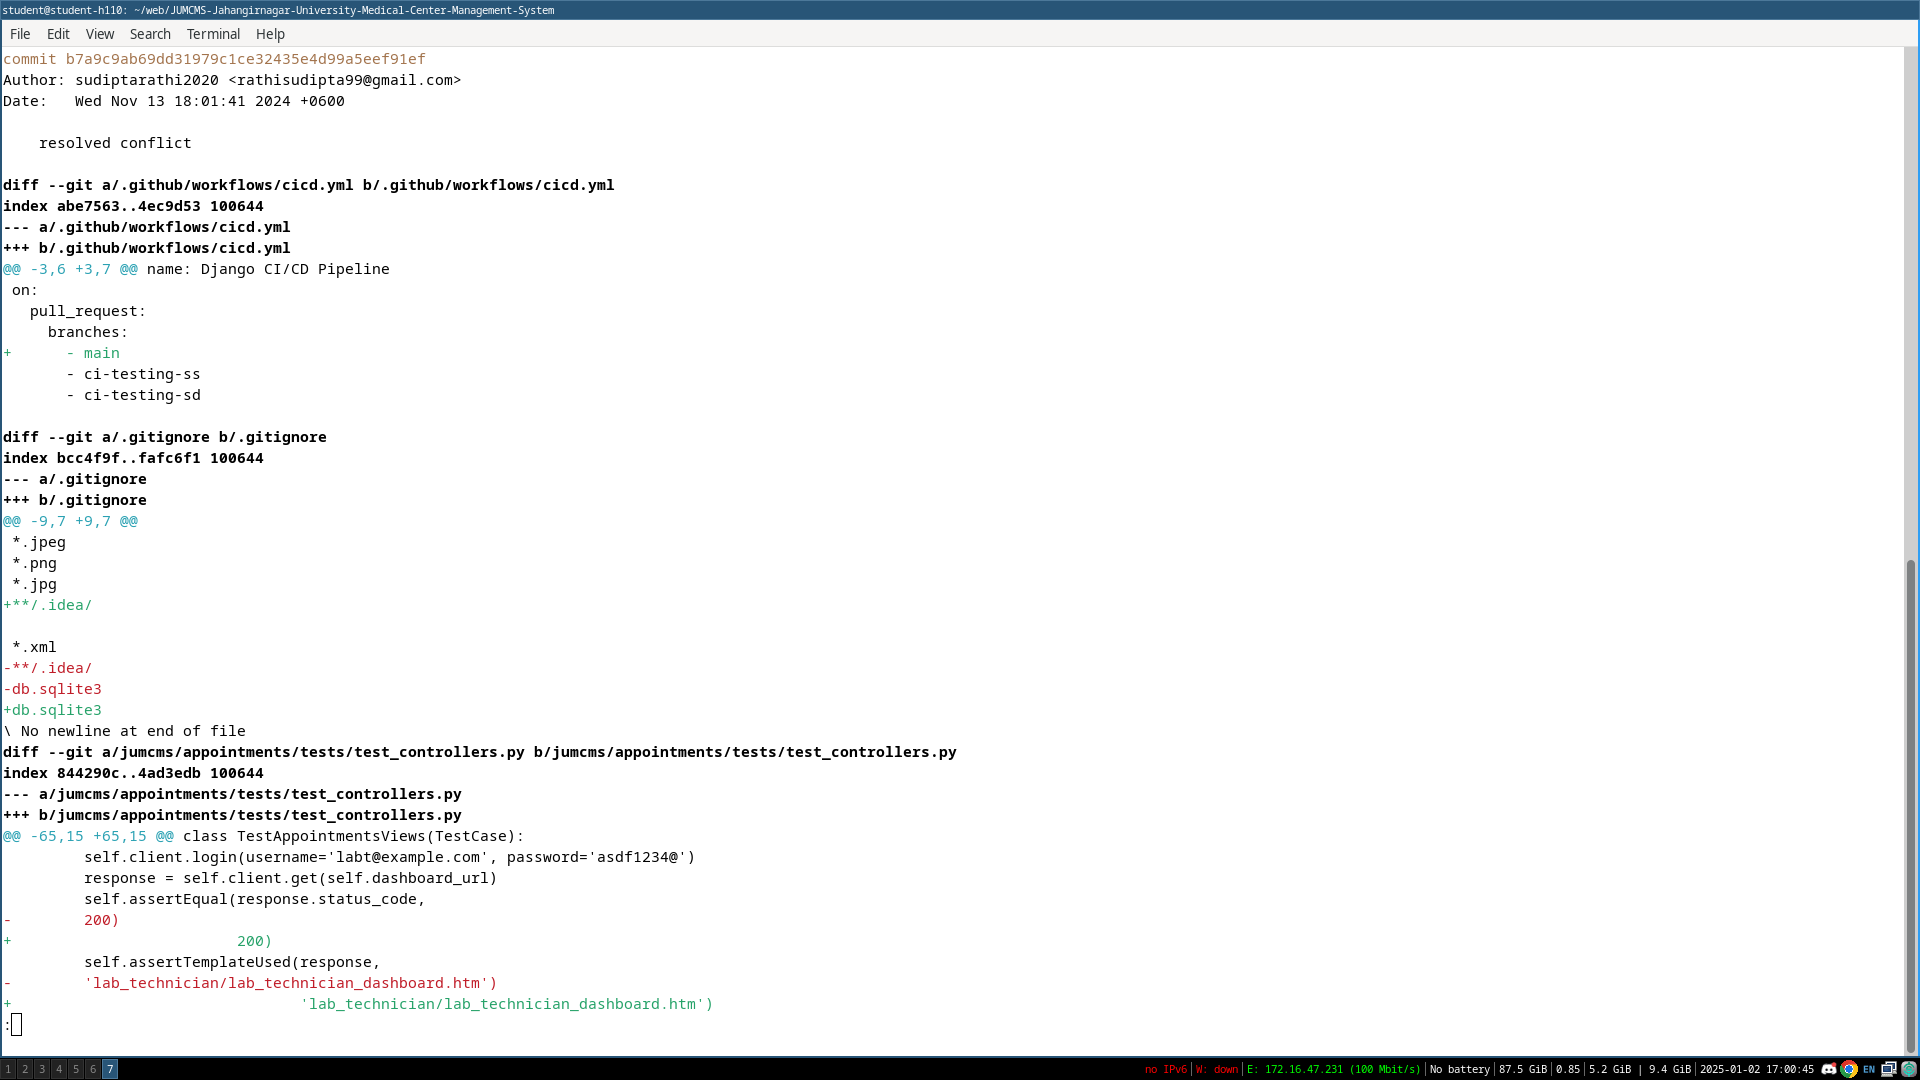
\includegraphics[width=1\textwidth]{images/meet45.png}
    \caption{git log}
    \label{fig:meet45}
\end{figure}

\begin{figure}[H]
    \centering
    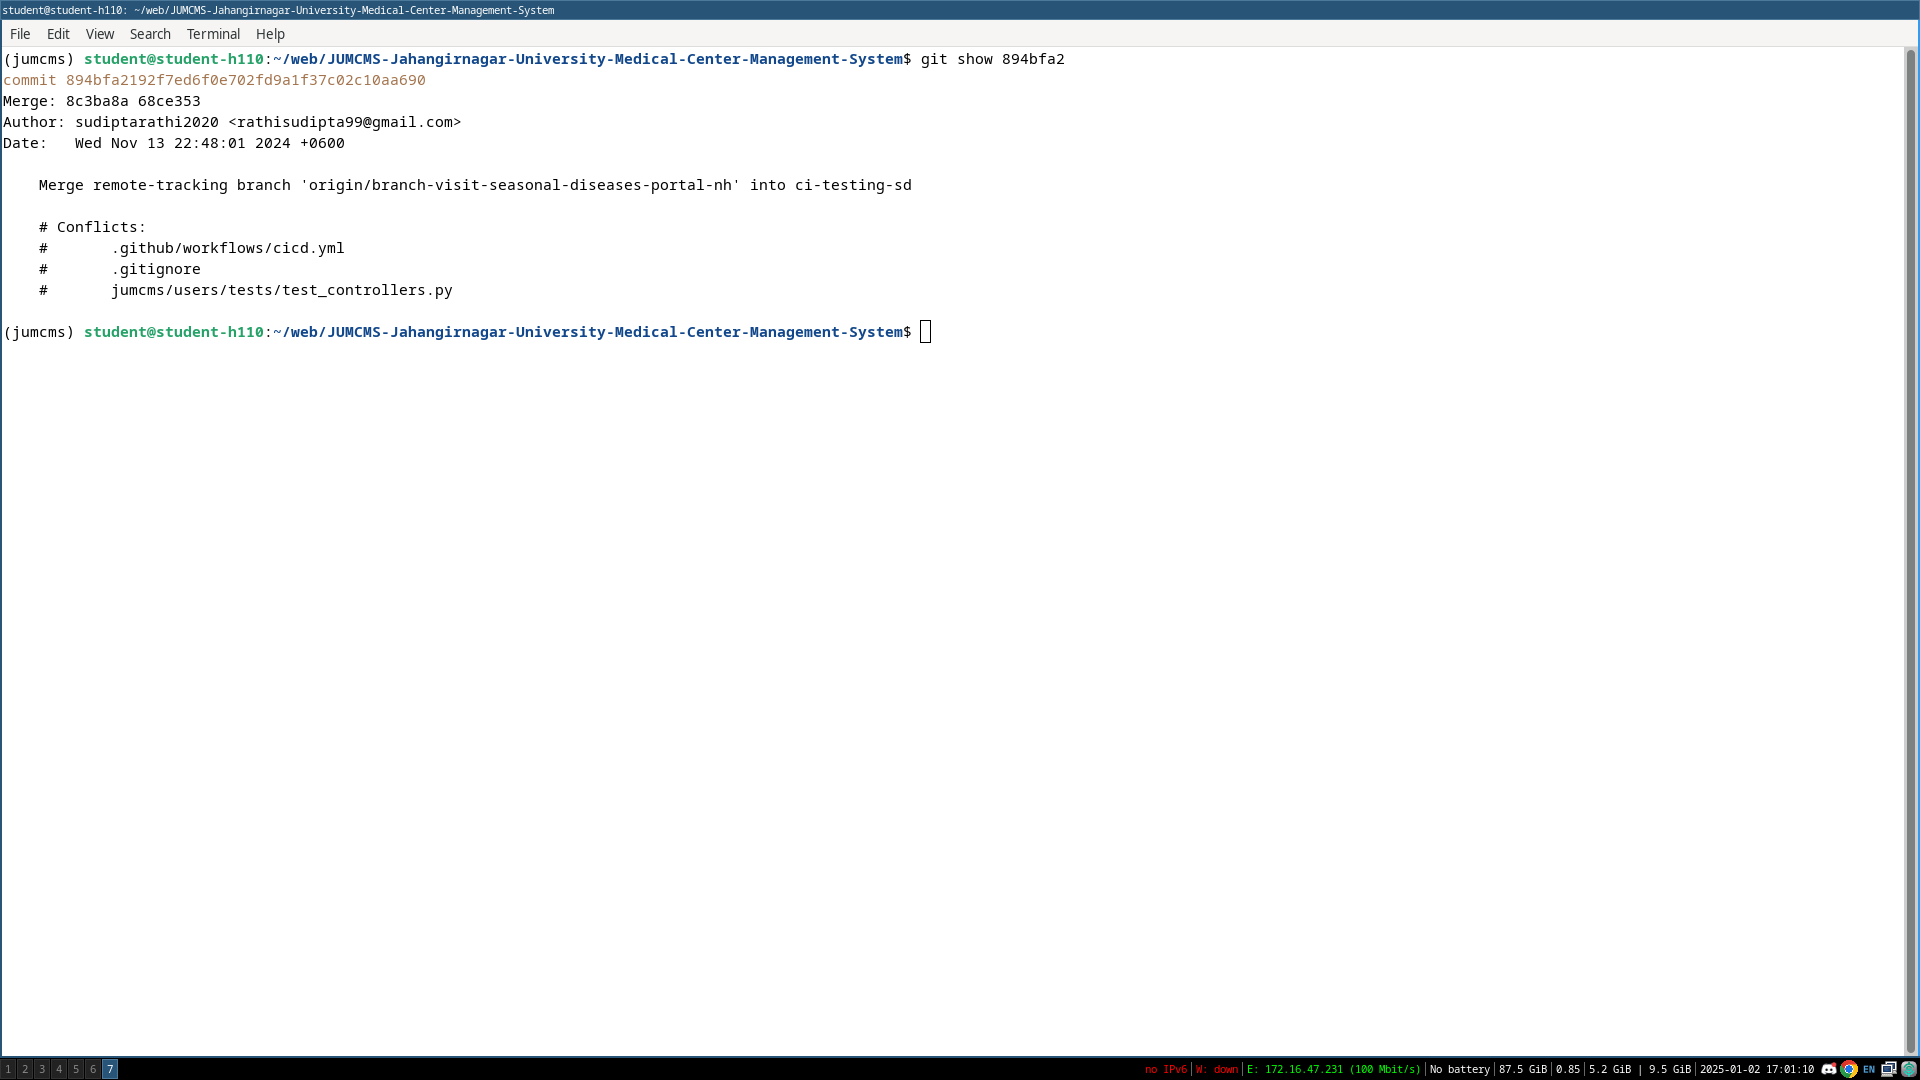
\includegraphics[width=1\textwidth]{images/meet46.png}
    \caption{git log}
    \label{fig:meet46}
\end{figure}

\begin{figure}[H]
    \centering
    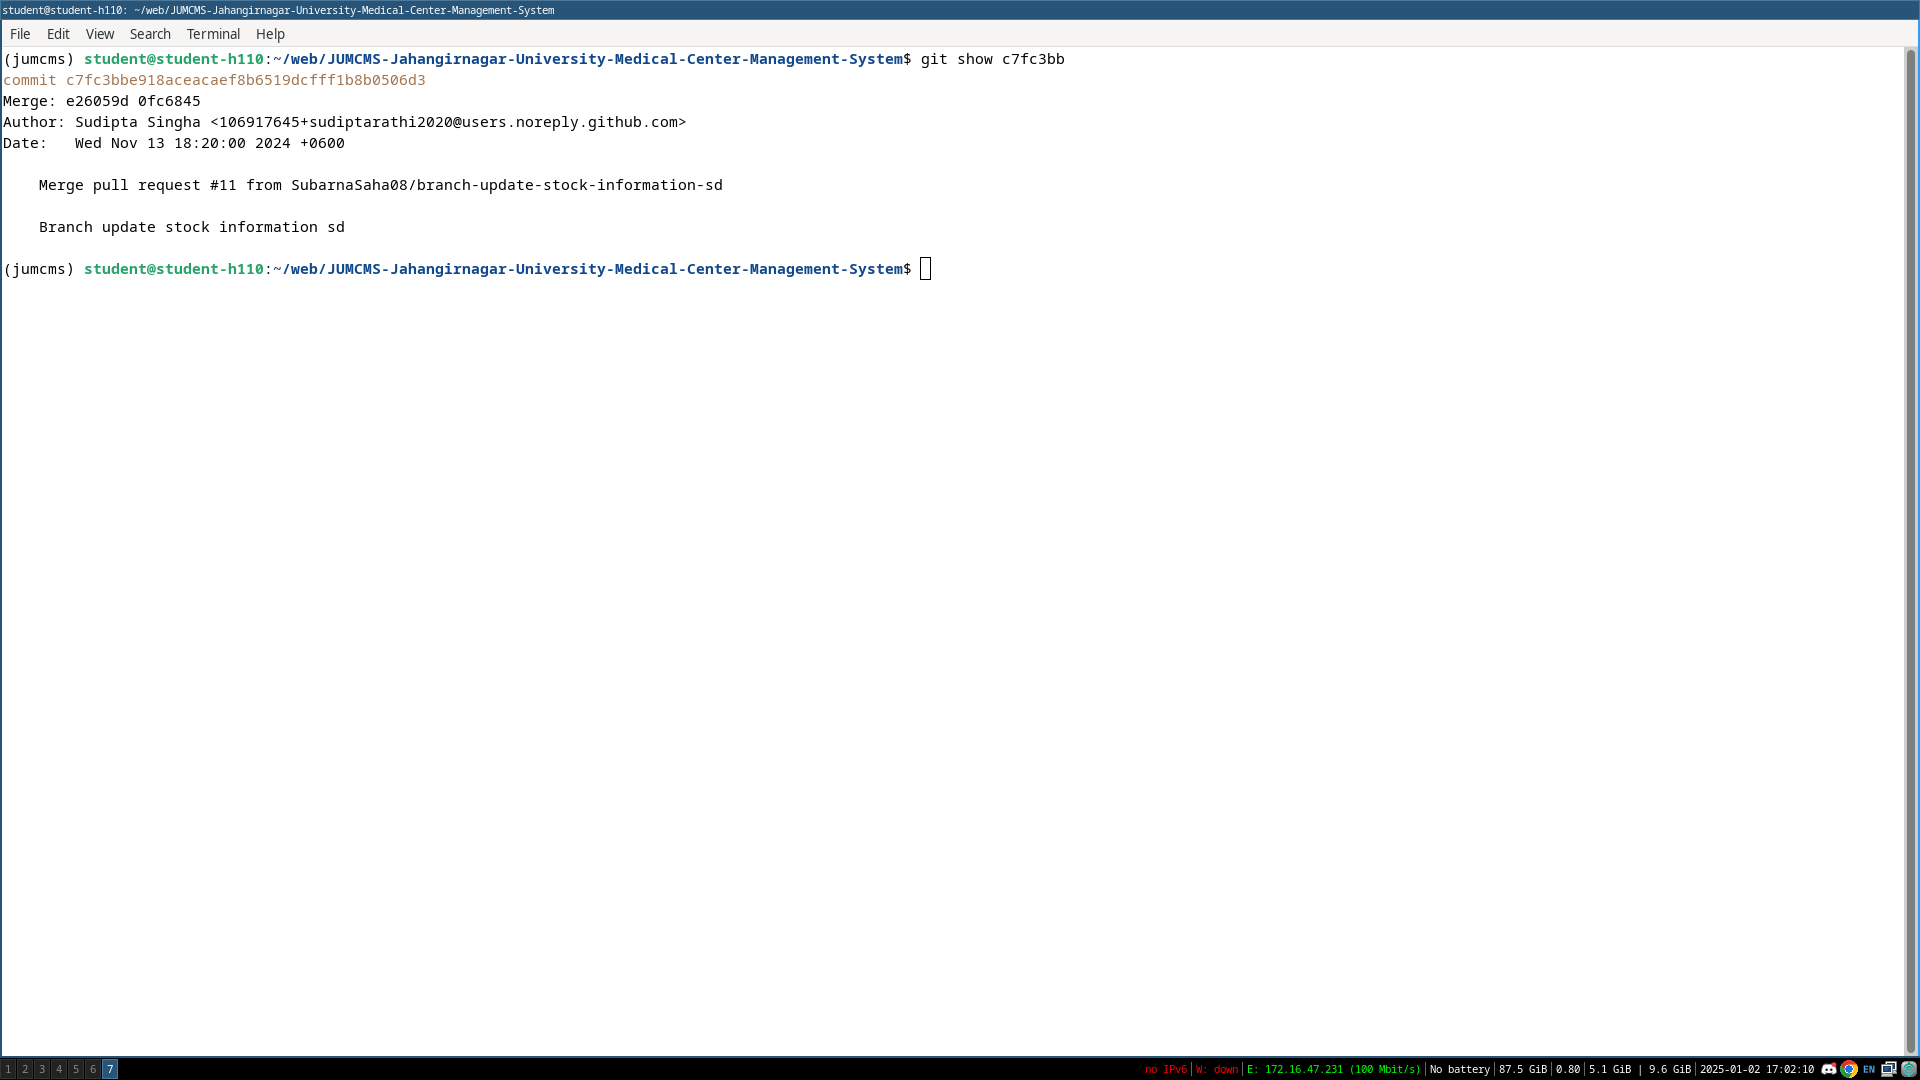
\includegraphics[width=1\textwidth]{images/meet47.png}
    \caption{git log}
    \label{fig:meet47}
\end{figure}

\begin{figure}[H]
    \centering
    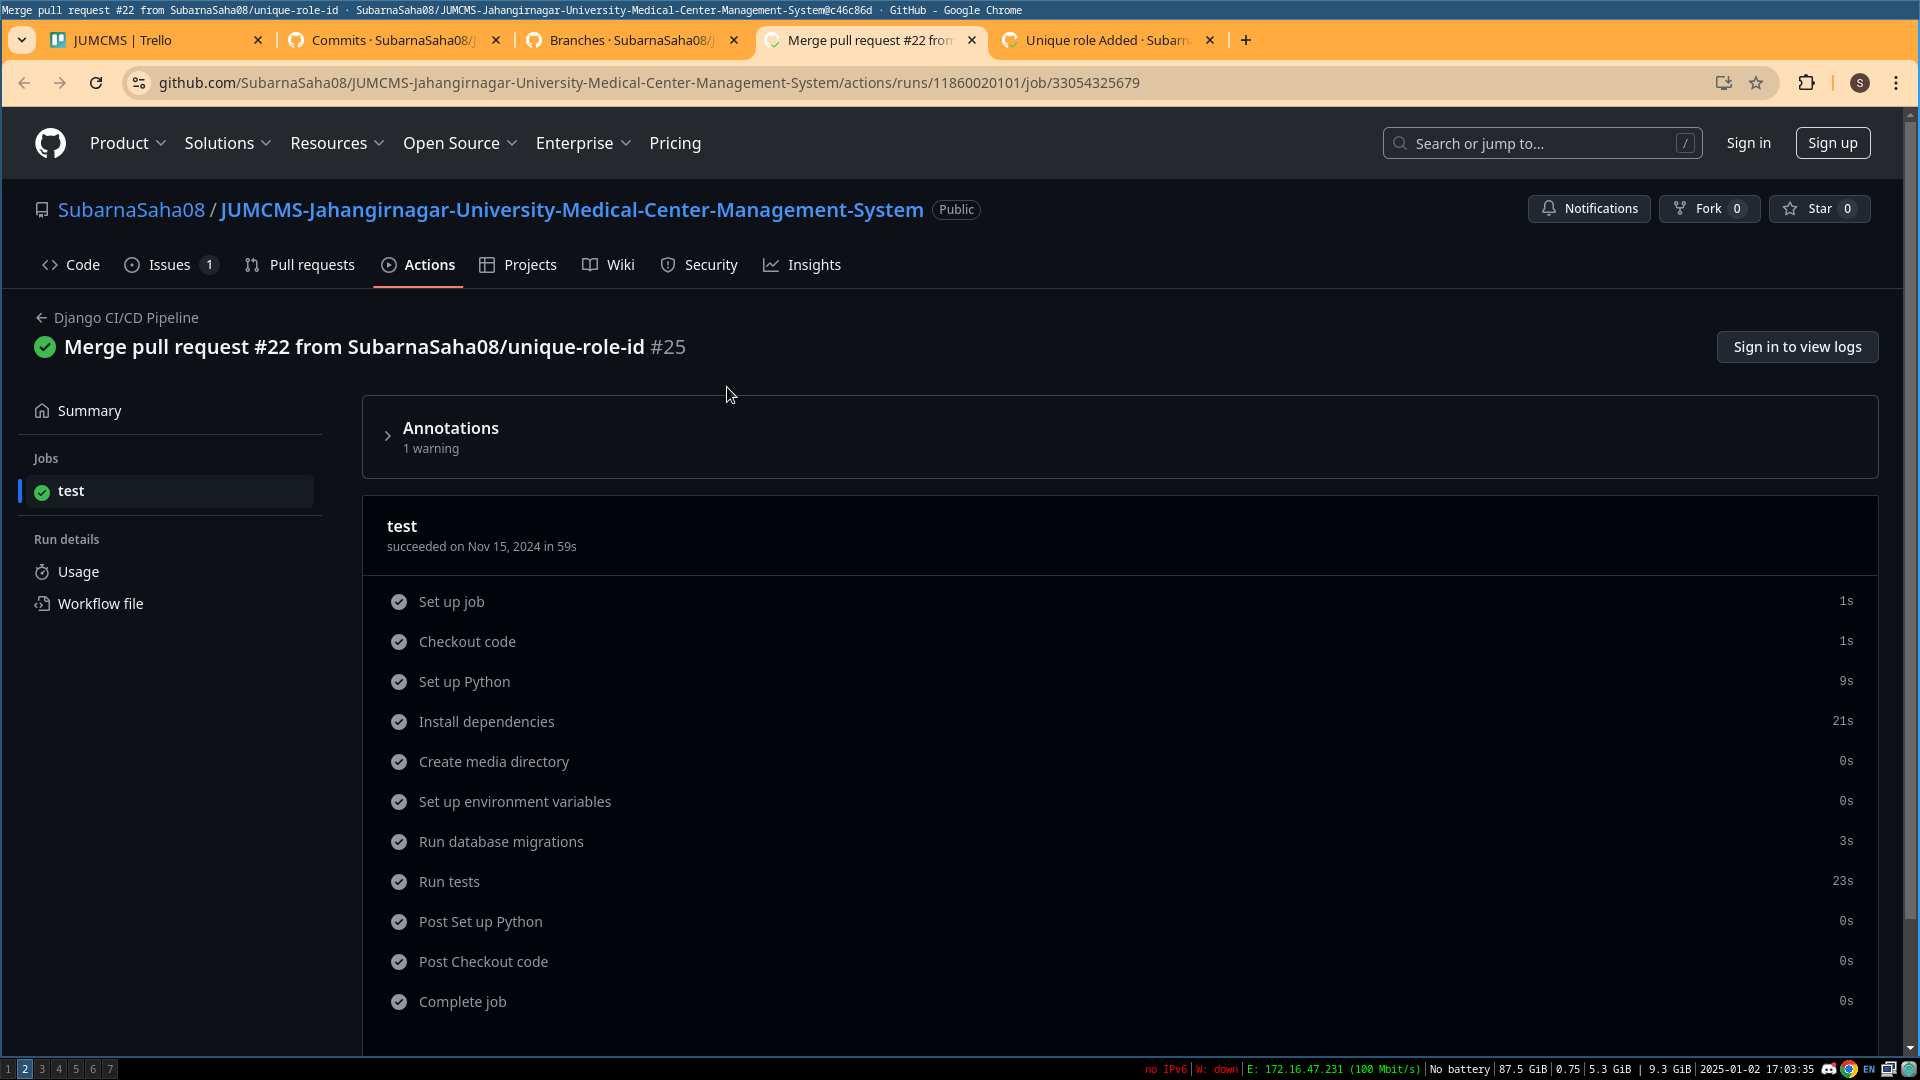
\includegraphics[width=1\textwidth]{images/meet48.png}
    \caption{CICD}
    \label{fig:meet48}
\end{figure}

\begin{figure}[H]
    \centering
    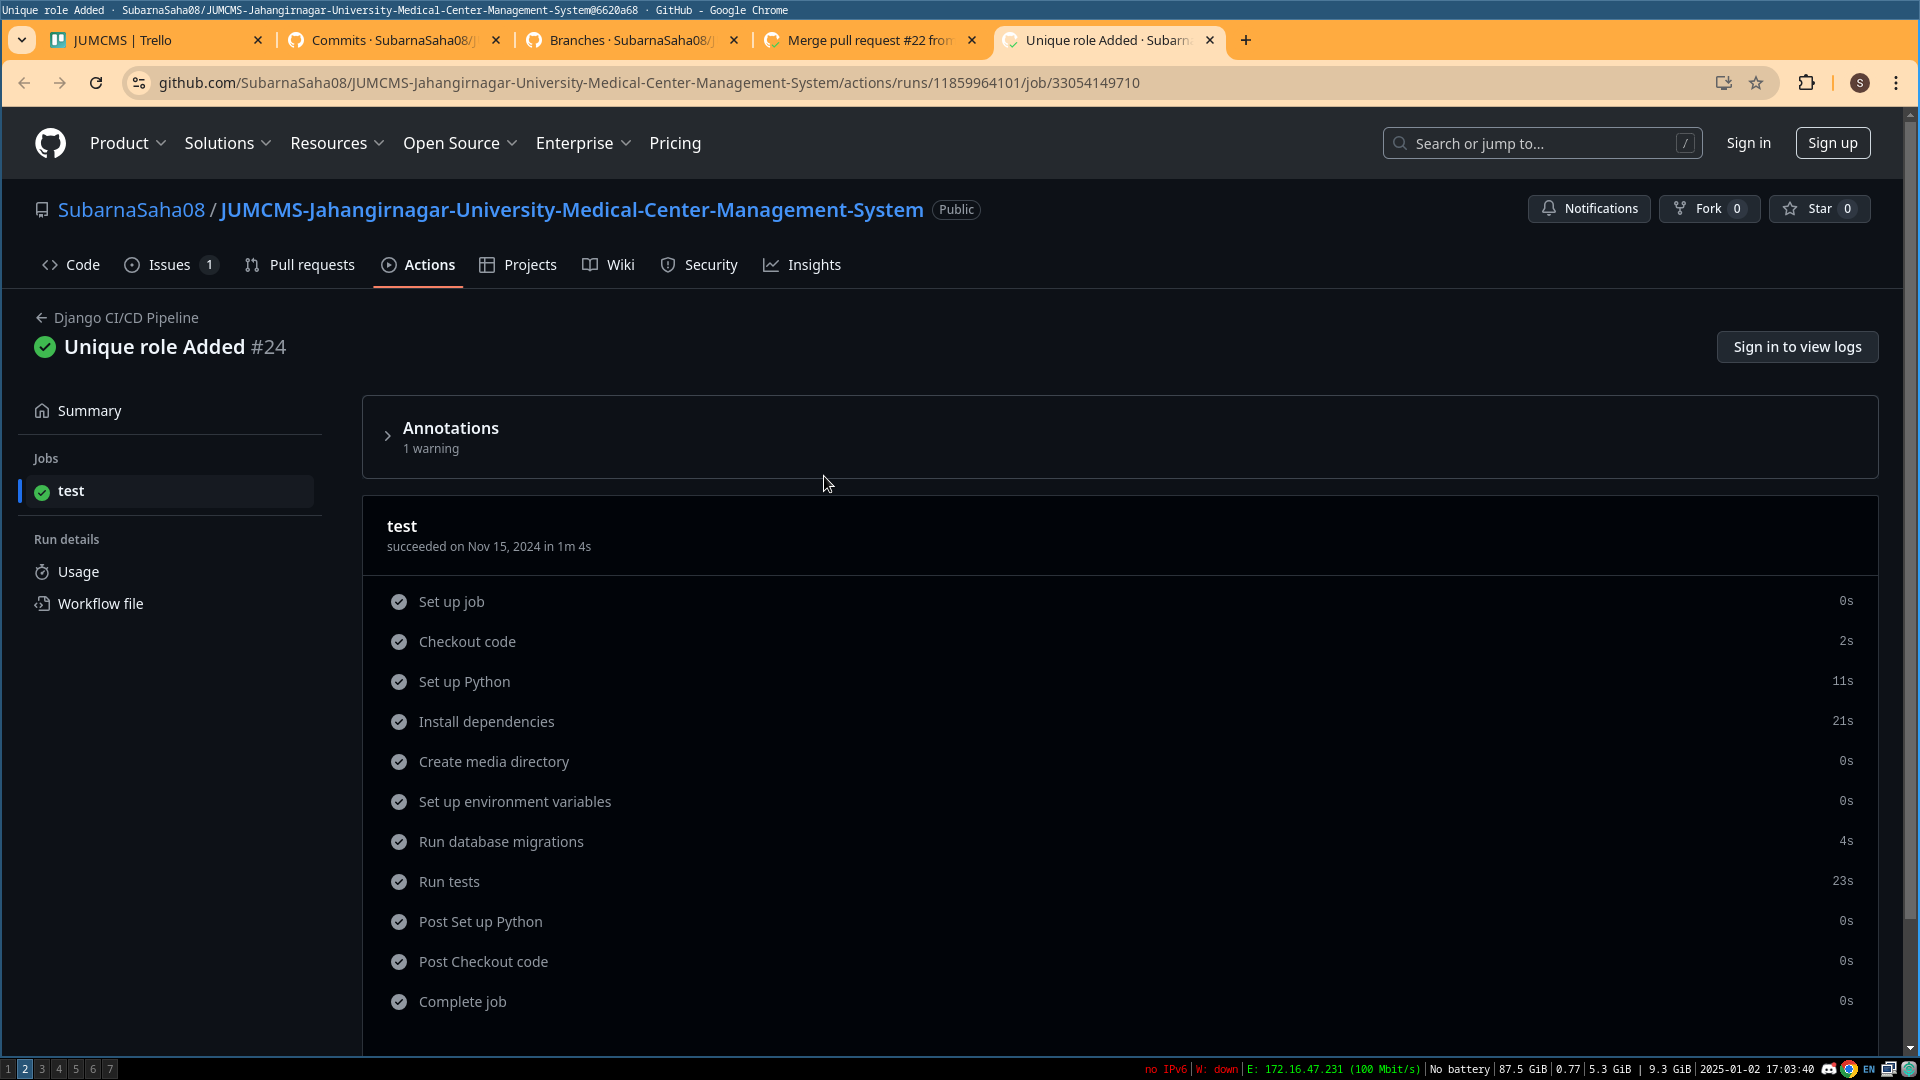
\includegraphics[width=1\textwidth]{images/meet49.png}
    \caption{CICD}
    \label{fig:meet49}
\end{figure}

\begin{figure}[H]
    \centering
    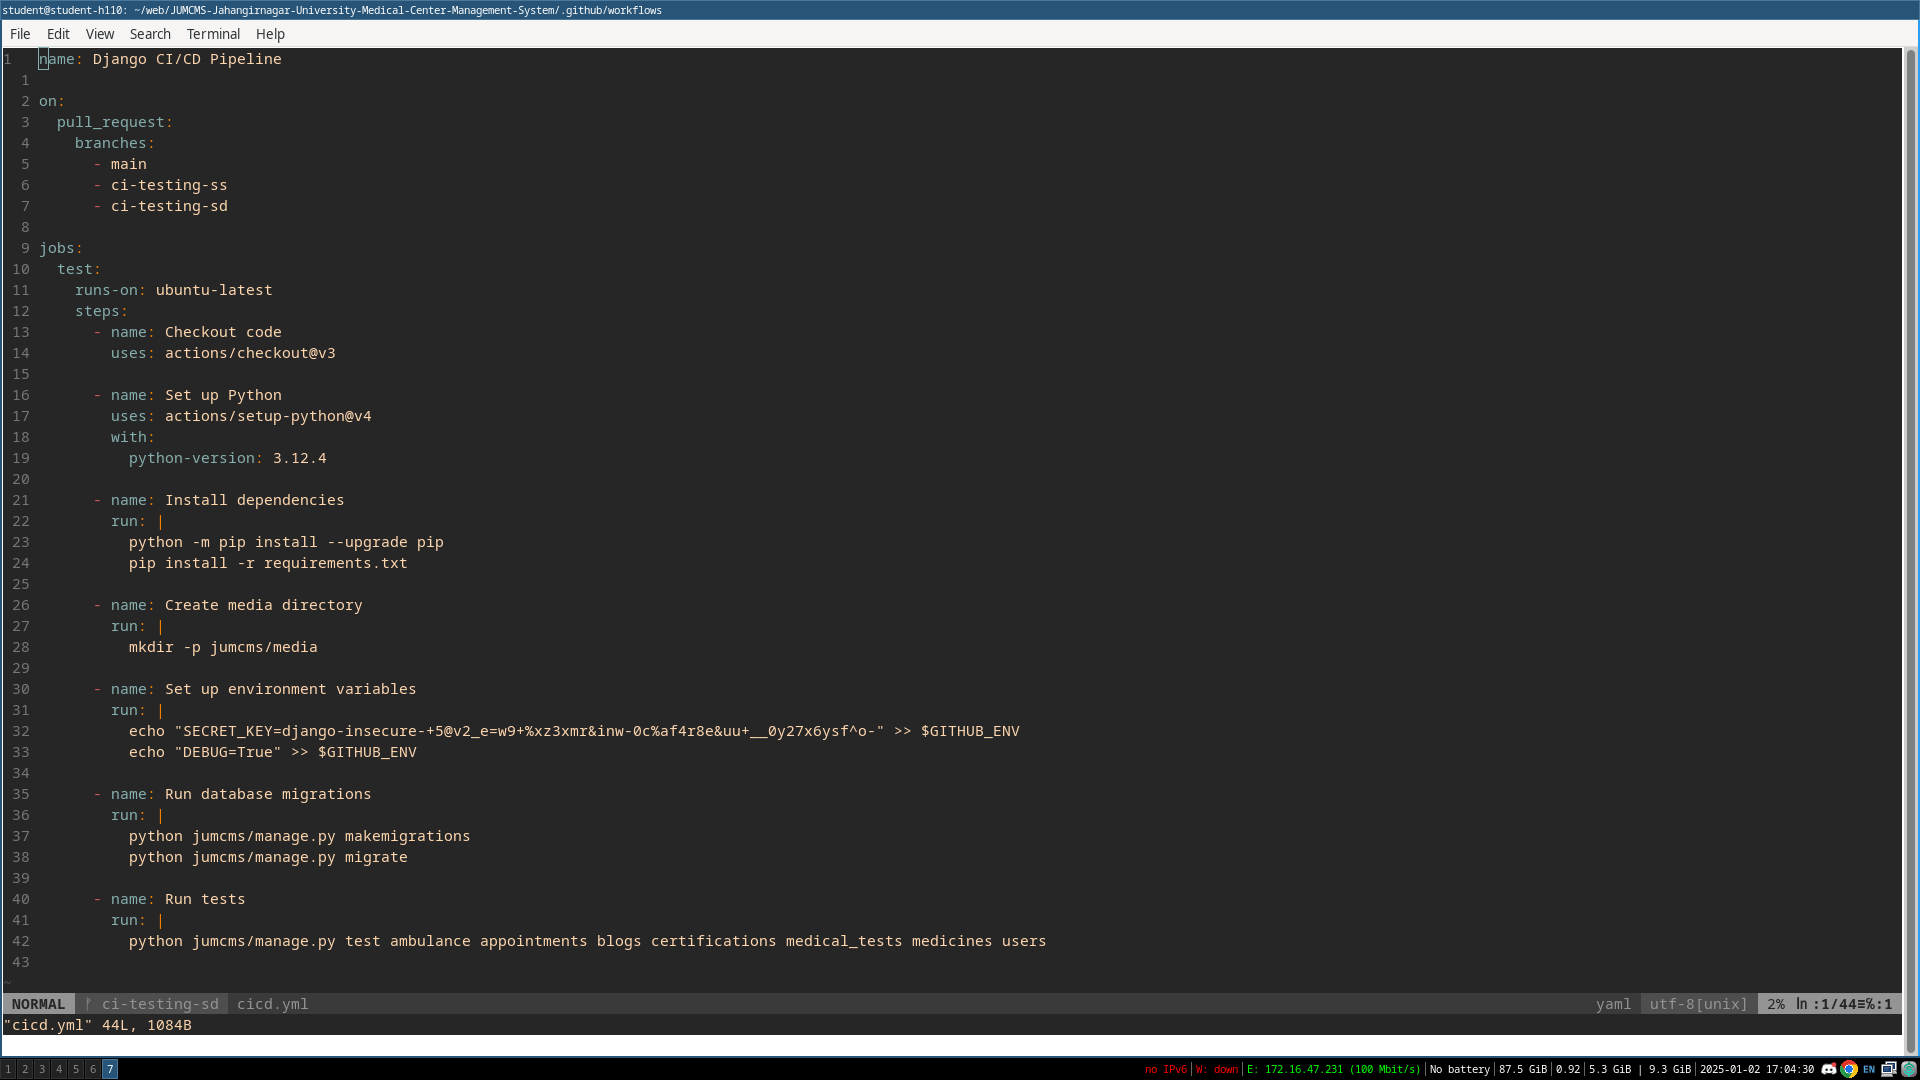
\includegraphics[width=1\textwidth]{images/meet410.png}
    \caption{cicd.yml file}
    \label{fig:meet410}
\end{figure}
\newpage
\subsection{Sprint Retrospective Meeting}
\textbf{What Went Well}
\begin{itemize}
    \item Discussing the positive aspects of the sprint, including achievements, successful teamwork, and processes that worked well.

    \item The TDD Approach of software development went smoothly.
    \item Completed Submit Test Report feature where lab technicians can submit test report of patients.
    \item Completed Collect Test Reports feature where patients can login to their dashboard and collect test reports which are submitted by lab technicians.
    \item Completed Prescribe Patients feature where doctor can prescribe medicines, suggest tests and give advice.
    \item Completed Certify For Fund-raise feature where admin can approve fund-raise applications.
    \item Completed Update Stock Information feature where storekeeper can update medicine stock information, add medicines to the store.
    \item Completed Visit The Seasonal Disease Portal where any user can see blogs published by admin.
    \item Tested all the implemented feature and all test were passed.
    \item Continuous Integration was successfully implemented using Github Actions.
    \item All branches were merged to main branch.
    \item Sphinx documentation was added successfully.
\end{itemize}
\textbf{What Could Be Improved}
\begin{itemize}
    \item Identifying areas for improvement, including challenges faced, bottlenecks, and aspects of the sprint that could be better.

    \item Faced some problems during branch merging. The merging procedure created a lot of conflicts, which are manually resolved.
    \item A proper .gitignore file was not implemented at first. Some pycache files are generated. Those pycache files created merge conflicts and takes some space in the repository.
    \item Faced some problems when adding sphinx documentation. But at the end sphinx documentation was properly added.
\end{itemize}
\textbf{Lessons Learned}
\begin{itemize}
    \item Capturing any key lessons learned from the sprint that can be applied to future sprints.

    \item Understood and practiced how "TDD" approach of software development works.
    \item Understood and practiced continuous integration using github actions.
\end{itemize}
\begin{figure}[H]
    \centering
    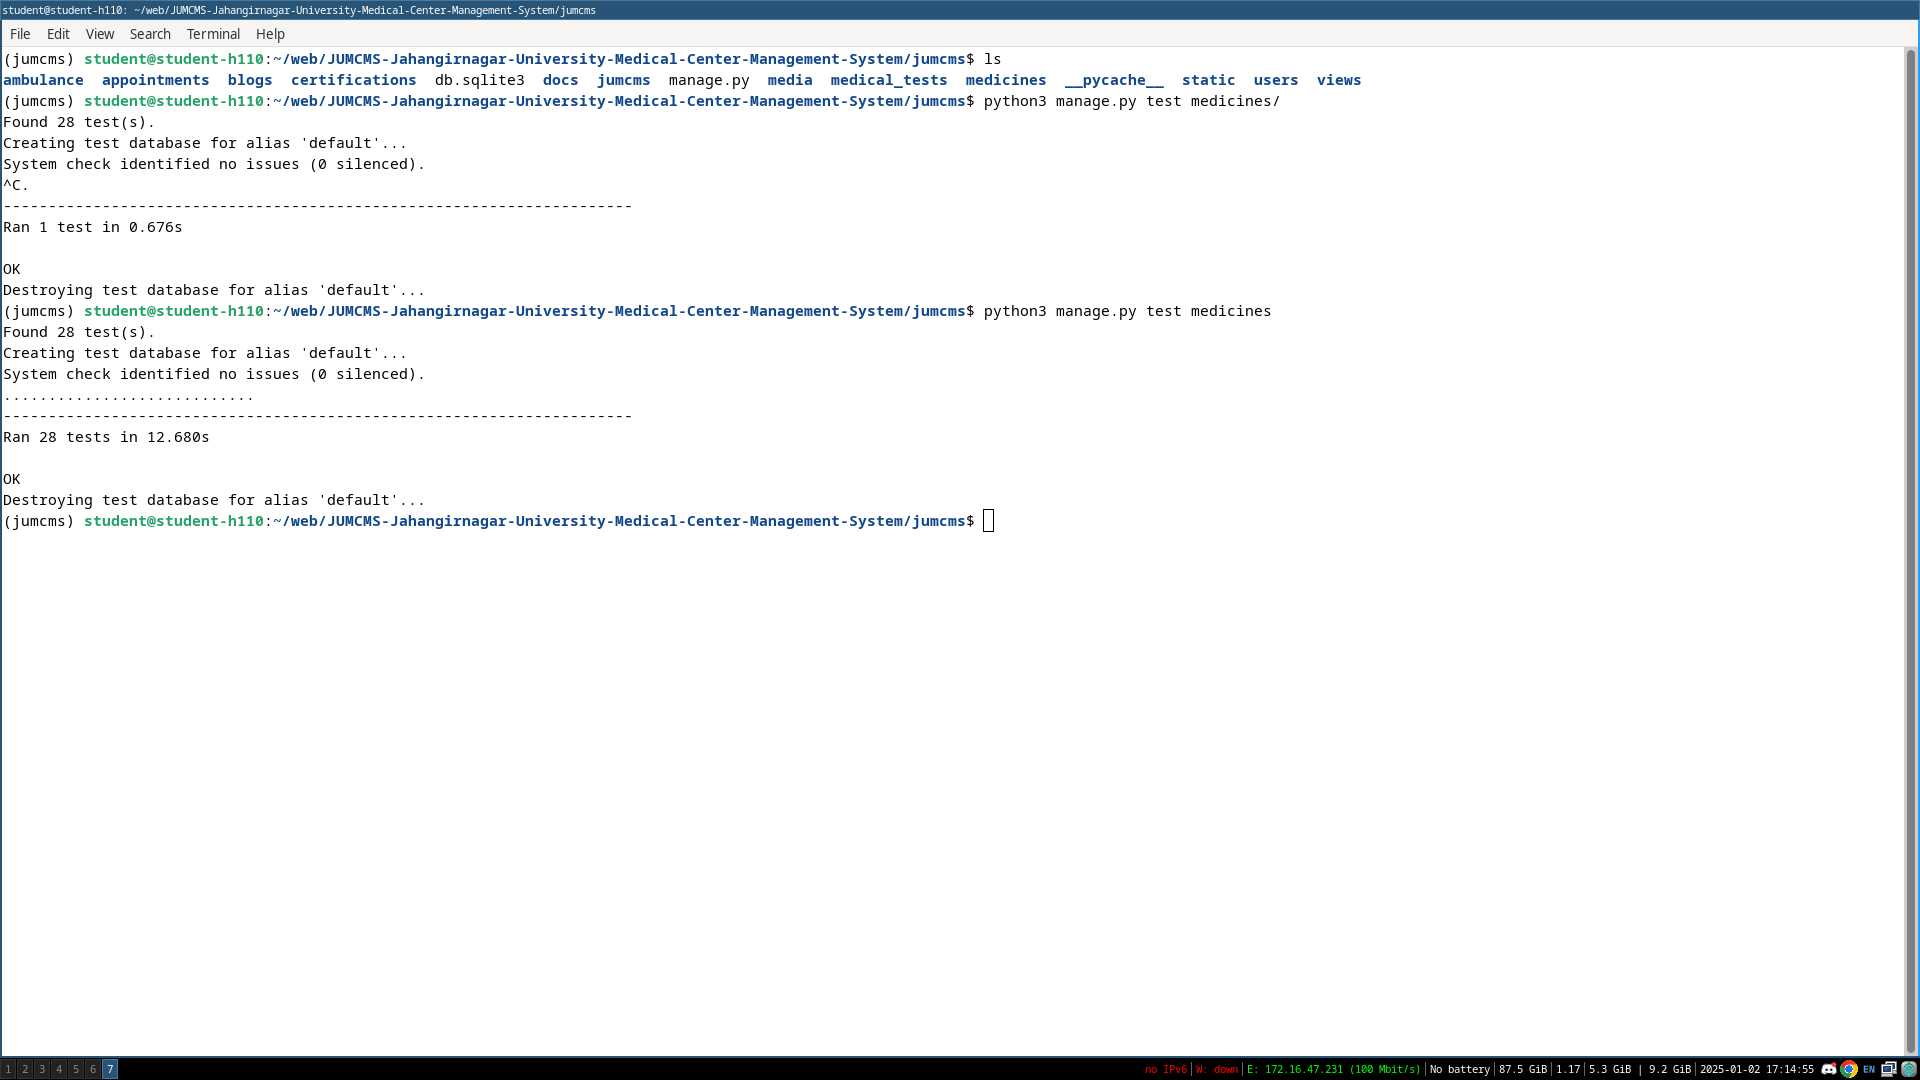
\includegraphics[width=1\textwidth]{images/meet4test.png}
    \caption{Test Case Passed}
    \label{fig:testcase}
\end{figure}
\begin{figure}[H]
    \centering
    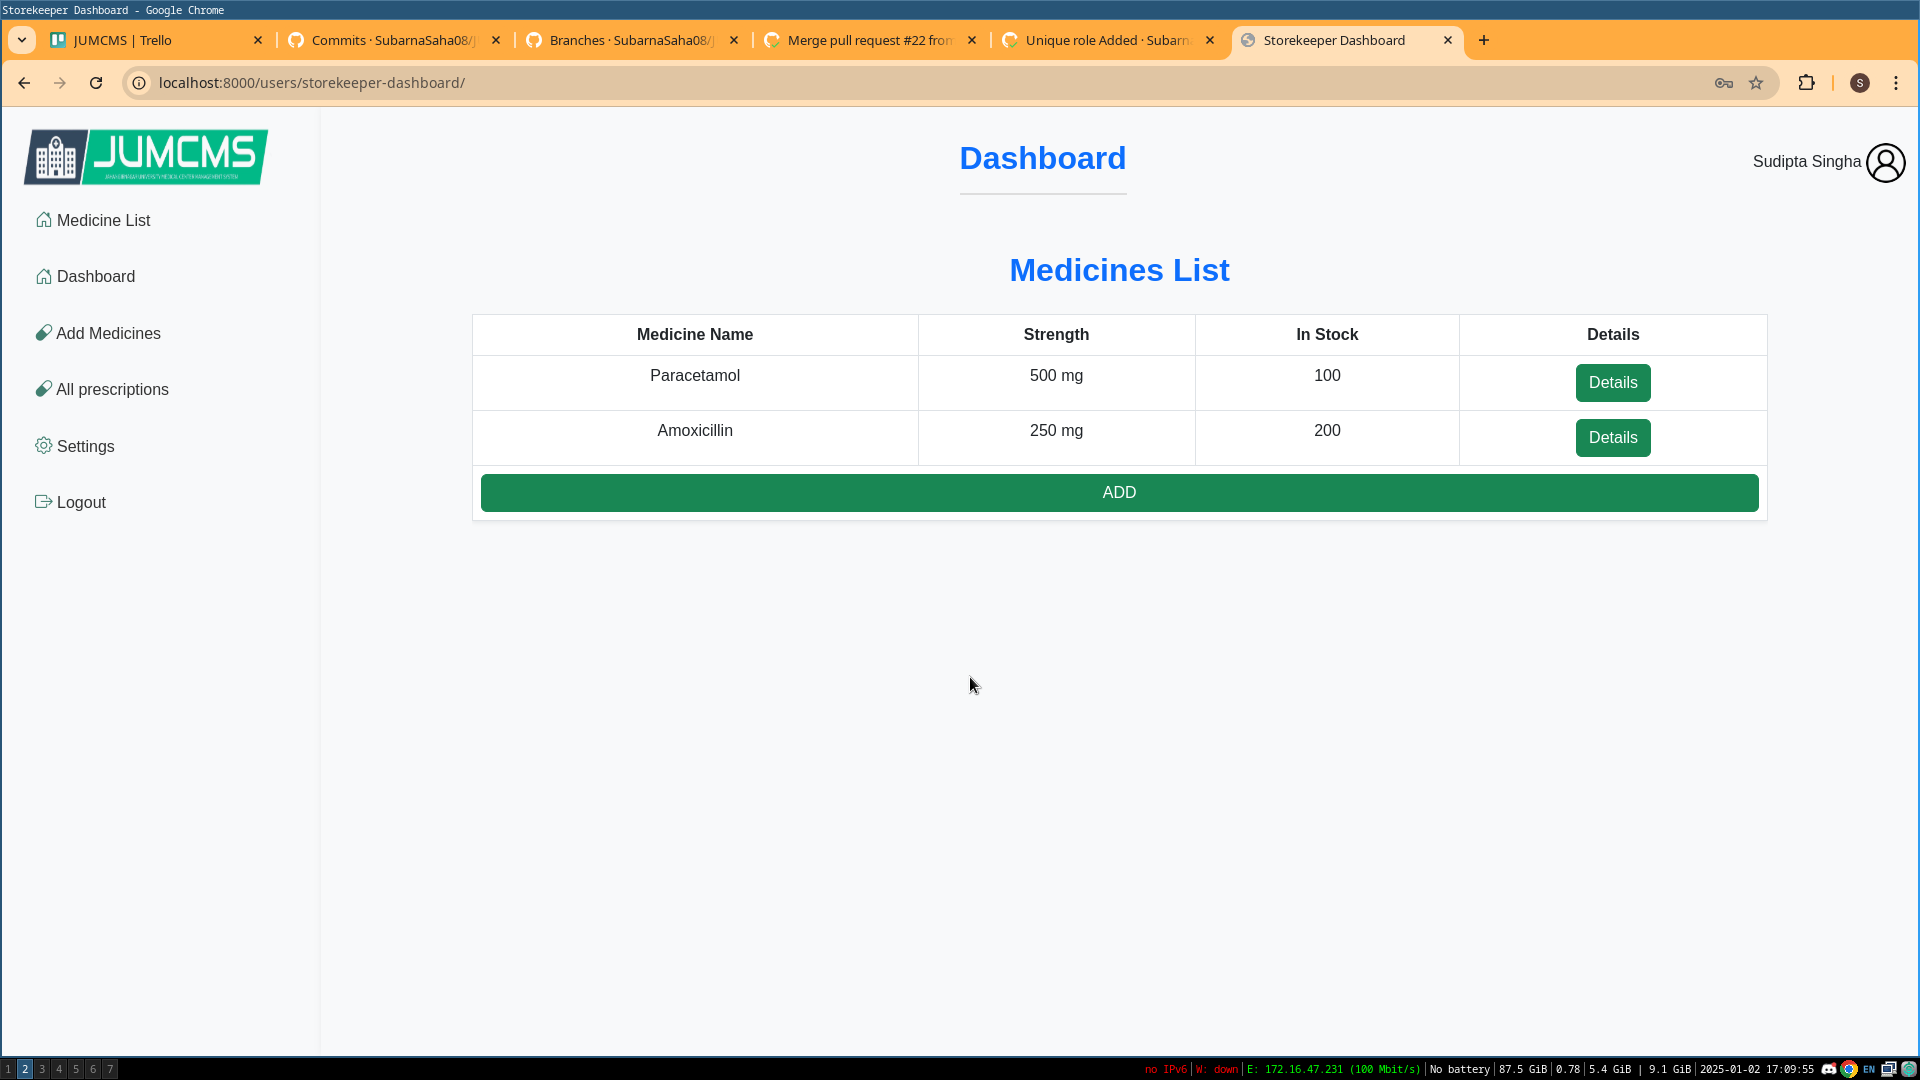
\includegraphics[width=1\textwidth]{images/output1.png}
    \caption{Output}
    \label{fig:output1}
\end{figure}
\begin{figure}[H]
    \centering
    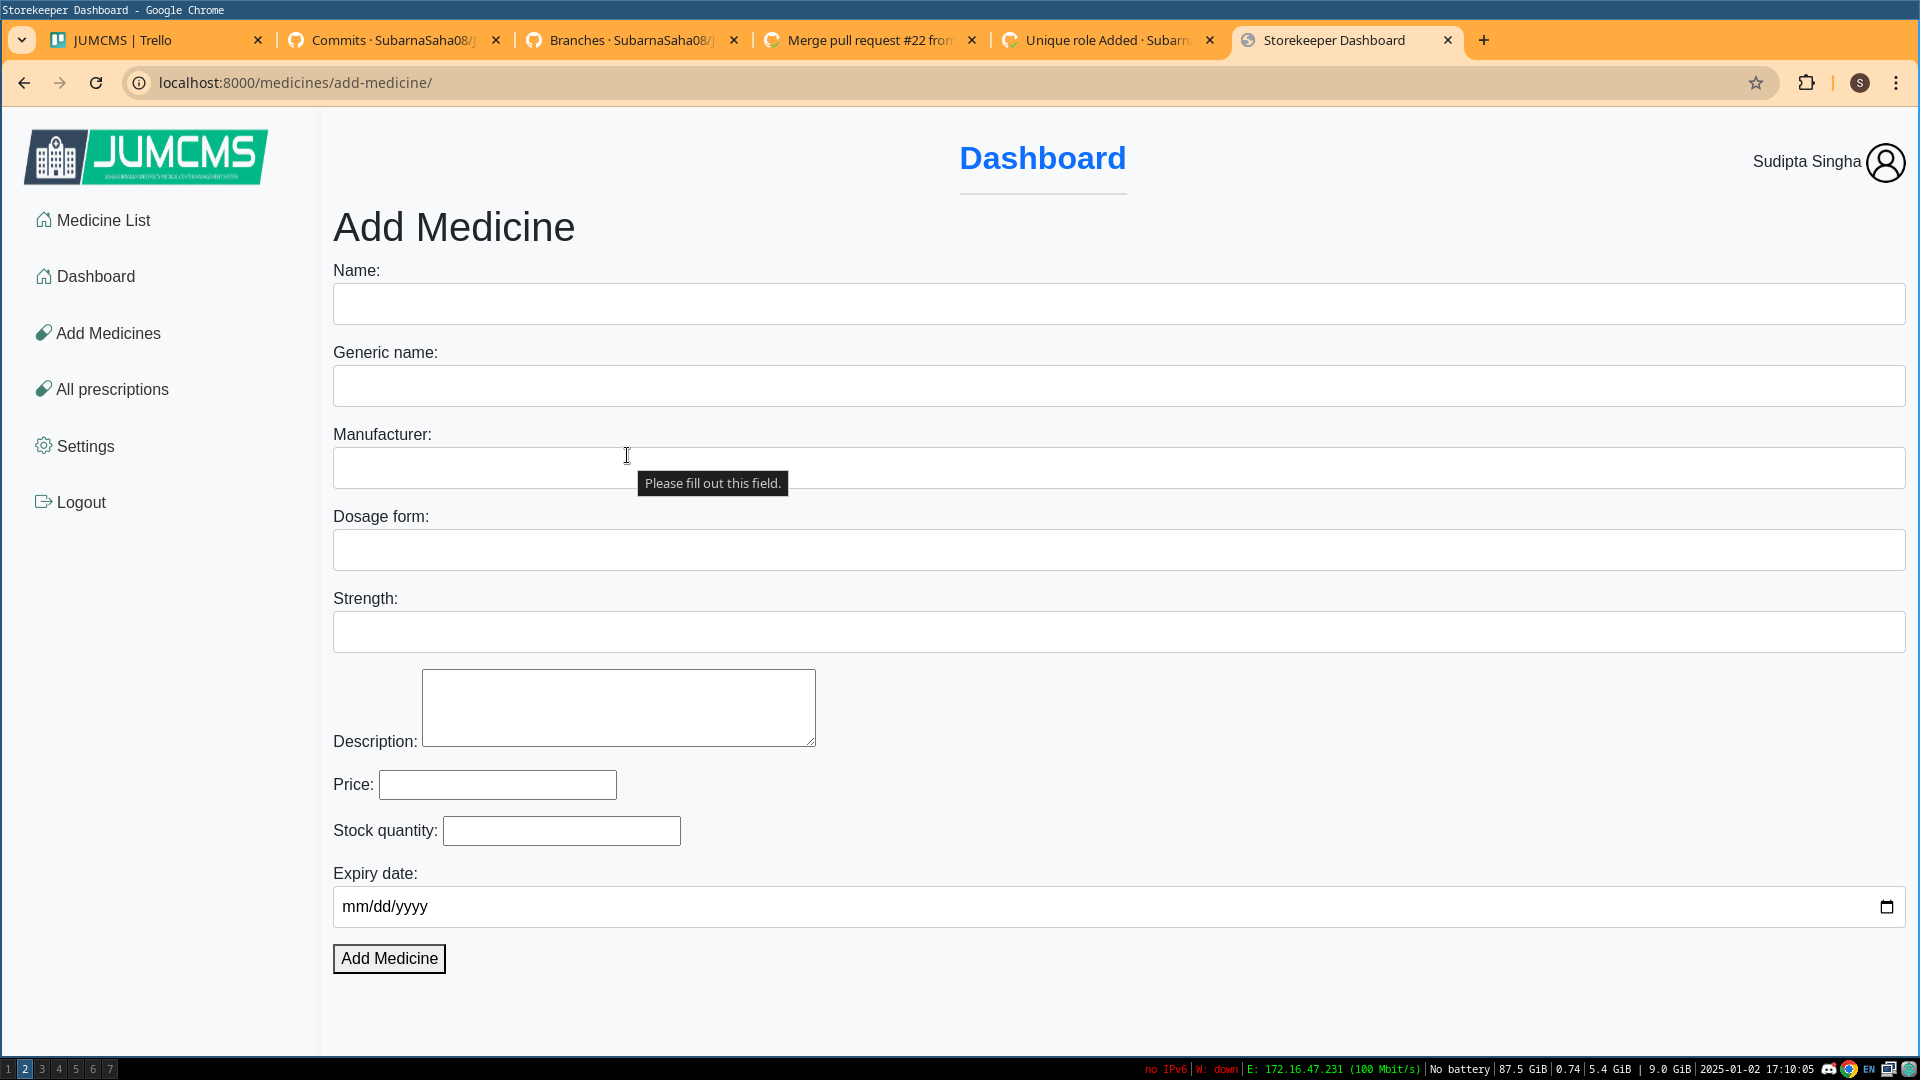
\includegraphics[width=1\textwidth]{images/output2.png}
    \caption{Output}
    \label{fig:output2}

\end{figure}
\begin{figure}[H]
    \centering
    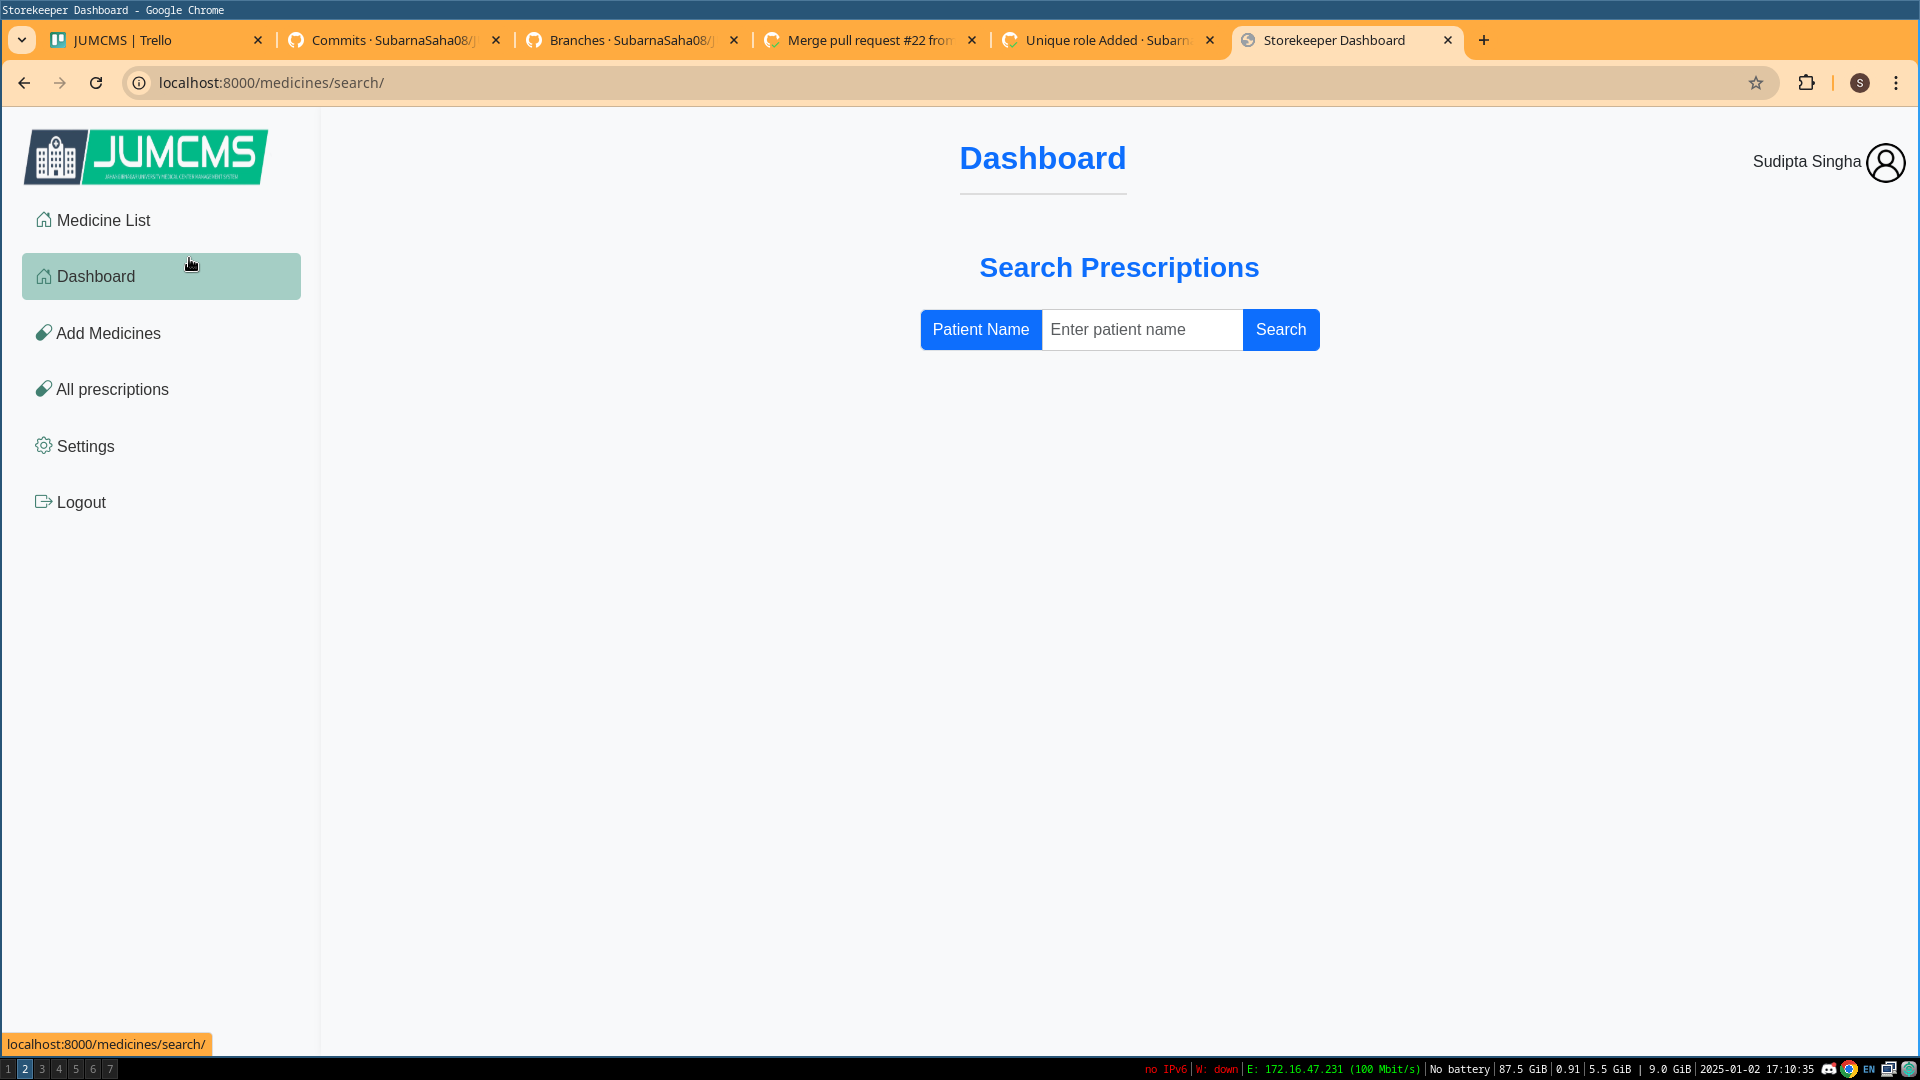
\includegraphics[width=1\textwidth]{images/output3.png}
    \caption{Output}
    \label{fig:output3}
\end{figure}
\end{document}
